\documentclass[12pt, english]{article}
\usepackage{graphicx}
\usepackage[colorlinks=true, linkcolor=blue]{hyperref}
\usepackage[english]{babel}
\selectlanguage{english}
\usepackage[utf8]{inputenc}
\usepackage[svgnames]{xcolor}

\usepackage{amsmath}
\usepackage{amsthm}
\usepackage{mathtools}
\usepackage{eucal}
\usepackage{amssymb}
\usepackage{mathrsfs}

\usepackage{listings}
\usepackage{afterpage}
\usepackage[font=small,labelfont=bf]{caption}
\pagestyle{plain}

\definecolor{dkgreen}{rgb}{0,0.6,0}
\definecolor{gray}{rgb}{0.5,0.5,0.5}
\definecolor{mauve}{rgb}{0.58,0,0.82}

\lstset{frame=tb,
language=Python,
aboveskip=4mm,
belowskip=4mm,
showstringspaces=false,
columns=flexible,
numbers=none,
keywordstyle=\color{blue},
numberstyle=\tiny\color{gray},
commentstyle=\color{dkgreen},
stringstyle=\color{mauve},
breaklines=true,
breakatwhitespace=true,
tabsize=3
}

\usepackage{here}
\usepackage{bm}


\textheight=21cm
\textwidth=17cm
\oddsidemargin=-.2cm
\pagestyle{plain}

\usepackage{color}
\usepackage{indentfirst}
\usepackage{ragged2e}

% Expectation symbol
\DeclareMathOperator*{\E}{\mathbb{E}}

\global\let\date\relax
\newcounter{unomenos}
\setcounter{unomenos}{\number\year}
\addtocounter{unomenos}{-1}
\stepcounter{unomenos}
\gdef\@date{ \arabic{unomenos} }

\usepackage[backend=bibtex,style=phys]{biblatex}
\bibliography{references} 

\begin{document}

\begin{titlepage}

\begin{center}
Wigner Research Center for Physics \\ Hungarian Academy of Sciences - \@date\\
\vspace*{0.5in}
\rule{150mm}{0.1mm}\\
\vspace*{0.3in}
\begin{Large}
\textbf{Interpreting hierarchical computations \\ in the visual cortex using\\ Deep Generative Models} \\
\end{Large}
\vspace*{0.3in}
\rule{150mm}{0.1mm}\\
\vspace*{0.4in}
\begin{large}
Alex Olar \\
\end{large}
\vfill
Computational Systems Neuroscience Lab \\
\vspace{2mm}

\includegraphics[width=2cm]{logoFAC.png}
\end{center}
\end{titlepage}

\newcommand{\CC}{C\nolinebreak\hspace{-.05em}\raisebox{.4ex}{\tiny\bf +}\nolinebreak\hspace{-.10em}\raisebox{.4ex}{\tiny\bf +}}
\def\CC{{C\nolinebreak[4]\hspace{-.05em}\raisebox{.4ex}{\tiny\bf ++}}}

\renewcommand{\thesection}{\Roman{section}.}
\renewcommand{\thesubsection}{\Roman{section}. \arabic{subsection}.}
\renewcommand{\thesubsubsection}{\Roman{section}. \arabic{subsection}.\arabic{subsection}.}

\tableofcontents
\newpage

\section{Introduction}

\vspace{7mm}

\subsection{General}

\vspace{7mm}

\par  The visual cortex is a hierarchically organized structure in the mammalian brain, in which the first computational layer (primary visual cortex - V1) is known to detect edges in visual stimuli \cite{hubel1968receptive}.
As the visual hierarchy ultimately produces the representation of high-level concepts such as objects, we have strong reasons to believe that the second computational layer (secondary visual cortex - V2) extracts features that are compositions of the edge features from V1, such as textures \cite{ZiembaV2}, although the representation in V2 is nowhere near as well-explored as the one in V1, and further levels of the visual hierarchy have been studied even less. In order to obtain a more complete understanding of the representational layers of the visual cortex, we need to build computational models that can take images as input and produce testable predictions about various measurable statistical properties of the neural activity elicited by the same images in human or animal brains \cite{yamins2014performance}.
While it is important that the variables of such models are comparable to experimentally recorded neurons, in order to provide a functional understanding of the visual system, they need to abstract away the biophysical details of neural and synaptic dynamics into abstract variables. For these reasons, we turn to computational models developed in machine learning, which have been highly successful in modelling image data, and apply them to provide insights to the computational architecture of the brain.

\vspace{4mm}

\par Since the brain is capable of behaving generatively, such as imagining things that do not exist from memory, therefore we should aim for developing such models. In this aspect, the latent representational models proved to be very good candidates such as the actively researched variational autoencoders (VAE) from the domain of deep learning \cite{kingma2013auto}. This model attempts to represent high-dimensional images in a smaller vector space with auxiliary constraints on the latent representation using deep neural networks.

\vspace{4mm}

\par There is a wealth of studies suggesting that the brain is doing probabilistic inference which requires that humans or other animals maintain an internal model of the world inside their brain, hence the latent code models. It is also suggested that this model is probabilistic. Since learning and inference in probabilistic models is only possible in constrained cases as most computations are intractable.

\vspace{7mm}

\subsection{Motivation}

\vspace{7mm}

\par The selection of this topic was motivated by the substantial development in neurobiology that could be achieved with the use and development of deep learning models. We could gather higher level information about the image-processing of the brain. It is important to mention that this research is on the border of different sciences such as information technology and neurobiology consequently it poses an exciting challenge to understand.

\vspace{4mm}

\par Recent advances in machine learning provide tools to tackle variational inference since VAEs perform approximate inference on complex data. Also biological insights can be used to explore several aspects of VAEs. Inspired by the hierarchical structure of the visual cortex, we seek to understand how hierarchical models can be built using VAEs. Some elementary but not trivial properties of images are tested, such as contrast and we explore how variational auto-encoders deal with them. These insights provide a way to see how a promising class of machine learning models can be used to get and understanding of visual processing in the mammalian visual cortex.

\vspace{7mm}

\subsection{Overview}

\vspace{7mm}

\par In the following essay we are going to present different models for understanding the visual cortex. Firstly, we will discuss early models such as sparse coding, since it was a breakthrough in getting a better insight on the V1. Moving on from this to current deep learning territory we are going to explain the details of auto-encoders, variational auto-encoders and ladder variational auto-encoders and their role in developing methods to understand the mammalian visual cortex. Variational inference used in VAEs and LVAEs is discussed in detail with the underlying theory and results. Moving on from theory we present details of the models used in this work heavily emphasizing that most components in the architectures can be freely swapped to lower or higher complexity ones. Additionally the main dataset is presented along with implementation details and nuances that made training of these deep neural networks successful in these settings. At last but not least in the results section contrast disentanglement is discussed in detail analyzing different models and input modifications in order to understand the acquired low-dimensional representations. 

\newpage

\section{Computational models}

\vspace{7mm}

\subsection{Early models}

\vspace{5mm}

\par It was the work of Olshausen and Field \cite{olshausen1996emergence} who proposed a model describing the structure of the first computational layer in the visual cortex (V1). The main assumption is that an image $I(x, y)$ can be decomposed on a set of linear basis functions:

\vspace{4mm}

\begin{equation}
    I(x, y) = \sum_{i}a_i \Phi_{i}(x, y)
\end{equation}

\vspace{4mm}

\par Where the components $a_{i}$ are pairwise decorrelated $\E (a_i a_j) = \E a_i \E a_j$. These assumptions were made to satisfy three main point:

\vspace{4mm}

\begin{itemize}
    \item spatially localized
    \item oriented
    \item bandpass - selective to structures at different scaled
\end{itemize}

\vspace{4mm}

\par PCA \footnote{Pricipal Component Analysis} was not fit for this type of problem since it provides a good tool for describing data where pairwise linear correlations are the most important form of statistical dependence. However, it is not the case for high-order correlations in natural images. In order to capture this they proposed a solution that minimizes entropy while sparsely coding the natural images, meaning that they wanted to describe each via a small set of variables out of the large set. The method developed is called sparse coding and a special case of it is ICA \footnote{Independent Component Analysis - \url{https://redwood.berkeley.edu/wp-content/uploads/2018/08/sparse-coding-ICA.pdf}}.

\vspace{5mm}

\subsection{VAE}

\vspace{5mm}

\par Auto-encoders are mostly used to reduce dimensionality of data in an unsupervised manner. They consist of an encoder and a decoder model surrounding the reduced representation \ref{fig:auto_encoder_scheme}. 

\vspace{4mm}

\begin{figure}[H]
    \centering
    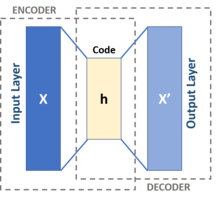
\includegraphics[width=0.3\linewidth]{220px-Autoencoder_schema.png}
    \caption{Basic scheme of an auto-encoder \footnote{From \url{https://en.wikipedia.org/wiki/Autoencoder}}}
    \label{fig:auto_encoder_scheme}
\end{figure}

\vspace{4mm}

\par These models are usually realized as neural networks due to their generalization capability as universal function approximators. Auto-encoders are a crucial tool for data compression and can reach better results than traditional algorithms \cite{theis2017lossy} such as lossy JPEG. Variational auto-encoders tackle the same problem while constraining the latent representation. This sacrifices reconstruction accuracy in order to learn a better representation of the used dataset.

\vspace{4mm}

\subsubsection{Variational inference in auto-encoders}

\vspace{4mm}

\par Considering a dataset $\boldsymbol{X} = \big\{\boldsymbol{\bm{x}}^{(i)}\big\}_{i = 1}^{N}$ that consists of independently and identically distributed samples of an underlying distribution $p{\boldsymbol{X}}$ it can be assumed that the data has some underlying, unobserved variable $\boldsymbol{\bm{z}}$. The value $\boldsymbol{\bm{z}}^{(i)}$, corresponding to a sample $\boldsymbol{\bm{x}}^{(i)}$, is first generated from a prior distribution $p_{\boldsymbol{\vartheta_{real}}}(\boldsymbol{\bm{z}})$ and $\boldsymbol{\bm{x}}^{(i)}$ is then generated from a conditional distribution $p_{\vartheta_{real}}(\boldsymbol{\bm{x}} | \boldsymbol{\bm{z}})$. Since the real model parameters $\vartheta_{real}$ are unknown we can only approximate them with the encoder and decoder parametric models. As we want to approximate the posterior probability:

\vspace{4mm}

\begin{equation}
    p_{\boldsymbol{\vartheta}}(\boldsymbol{\bm{z}} | \boldsymbol{\bm{x}}) \propto p_{\boldsymbol{\vartheta}}(\boldsymbol{\bm{x}} | \boldsymbol{\bm{z}}) p_{\boldsymbol{\vartheta}}(\boldsymbol{\bm{z}})
\end{equation}

\vspace{4mm}

\par Where basically we just applied Bayes-theorem for the likelihood and the prior to acquire the posterior \footnote{the true posterior is intractable since it would require us to calculate $p_{\vartheta}(\bm{x})$}. We build an encoder/recognition model $q_{\phi}(\boldsymbol{\bm{z}} | \boldsymbol{\bm{x}})$ and a decoder model $p_{\vartheta}(\boldsymbol{\bm{x}} | \boldsymbol{\bm{z}})$. The probabilistic encoder produces a distribution over $\boldsymbol{\bm{z}}$ that should properly approximate the prior while the  decoder provides samples from the approximated true distribution given a latent code. This is obviously a two-step generation process. 

\vspace{4mm}

\par In the article of Kingma and Welling \cite{kingma2013auto} they present a variational model that can be trained with gradient descent including stochastic variables. This is not a straigthforward problem since back-propagation through stochastic layers is not possible by default. They achieve this goal as explained here:

\vspace{4mm}

\begin{gather*}
    recognition\ model\ :\  q_{\phi}(\bm{z}|\bm{x}) \xrightarrow{\text{approximates}} p_{\vartheta_{real}}(\bm{z} | \bm{x}) \\
    probabilistic\ decoder\ :\ p_{\vartheta}(\bm{x} | \bm{z}) \xrightarrow{\text{approximates}} p_{\vartheta_{real}}(\bm{x} | \bm{z})
\end{gather*}

\vspace{4mm}

\par As the data points from the dataset are independent $p(\bm{x}^{(1)}, \bm{x}^{(2)}, ..., \bm{x}^{(N)}) = p(\bm{x}^{(1)})p(\bm{x}^{(2)})\cdot ... \cdot p(\bm{x}^{(N)})$ we can apply everything on $p(\bm{x}^{(i)})$, so approximating $p(\bm{x}^{(i)})$ in general can be calculated as follows:

\vspace{4mm}

\begin{gather}
    \ln p(\bm{x}^{(i)}) = \ln\int p(\bm{x}^{(i)}, \bm{z})dz \quad from\ marginal\ prob.\ dist.\\
    \ln p(\bm{x}^{(i)}) = \ln\int p(\bm{x}^{(i)}, \bm{z})\frac{q(\bm{z})}{q(\bm{z})}dz \quad introducing\ the\ prior \\
    \ln p(\bm{x}^{(i)}) = \ln \E_{q(\bm{z})} \Big( \frac{p(\bm{x}^{(i)}, \bm{z})}{q(\bm{z})}\Big) \\
    \ln \E_{q(\bm{z})} \Big( \frac{p(\bm{x}^{(i)}, \bm{z})}{q(\bm{z})}\Big) \geq \E_{q(\bm{z})} \ln\Big( \frac{p(\bm{x}^{(i)}, \bm{z})}{q(\bm{z})}\Big) \quad applying\ Jensen's\ inequality \\
    L_{i} = \ln p(\bm{x}^{(i)}) \geq \E_{q(\bm{z})} \ln\Big( \frac{p(\bm{x}^{(i)}, \bm{z})}{q(\bm{z})}\Big) \quad ELBO
\end{gather}

\vspace{4mm}

\par Jensen's inequality holds for convex functions and the natural logarithm is such. By applying the definition of the joint probability term $p(\bm{x}, \bm{z}) = p(\bm{x} | \bm{z})p(\bm{z})$ and realizing that we use the recognition model for $q(\bm{z})$ in our case $q_{\phi}(\bm{z} | \bm{x})$:

\vspace{4mm}

\begin{equation}
    L_{i} \geq \E_{q_{\phi}(\bm{z} | \bm{x})} \Big( \ln p(\bm{x}^{(i)} | \bm{z}) \Big) + \E_{q_{\phi}(\bm{z} | \bm{x})} \Big( \ln p_{\vartheta}(\bm{z} | \bm{x}^{(i)}) \Big) - \E_{q_{\phi}(\bm{z} | \bm{x})} \Big( \ln q_{\phi}(\bm{z} | \bm{x}^{(i)}) \Big)
\end{equation}

\vspace{4mm}

\par By introducing the Kullback-Leibler-divergence term that in layman's term measures the difference of two probability distributions therefore in optimization it ensures that two distributions should be close to each other:

\vspace{4mm}

\begin{gather*}
    KL(q_{\phi}(\bm{z} | \bm{x}^{(i)}) | p_{\vartheta}(\bm{z} | \bm{x}^{(i)})) = \int q_{\phi}(\bm{z} | \bm{x}^{(i)})\ln \frac{q_{\phi}(\bm{z} | \bm{x}^{(i)})}{p_{\vartheta}(\bm{z} | \bm{x}^{(i)})}dz = \E_{q_{\phi}(\bm{z} | \bm{x}^{(i)})} \Big( \ln \frac{q_{\phi}(\bm{z} | \bm{x}^{(i)})}{p_{\vartheta}(\bm{z}|\bm{x}^{(i)})}  \Big) \\ \\
    KL(q_{\phi} | p_{\vartheta}) = -L_{i} + \E_{q_{\phi}(\bm{z} | \bm{x}^{(i)})} \Big( \ln p_{\vartheta}(\bm{x}^{(i)} | \bm{z}) \Big) \quad using\ Bayes-theorem
\end{gather*}

\vspace{4mm}

\par The goal of the algorithm is to optimize the variational lower bound (ELBO) with respect to the parameters $\phi, \vartheta$. We also introduce $p_{\vartheta}(\bm{z} | \bm{x}^{(i)}) \equiv p_{\vartheta}(\bm{z})$, for all data points, as our prior distribution over the latent variables. Since the gradient of the ELBO is a bit problematic, especially requiring a large amount of computation w. r. t. $\phi$, Kingma and Welling came up with auto-encoding variational Bayes (AEVB) algorithm that makes the model trainable via stochastic gradient descent.

\vspace{4mm}

\paragraph{The reparametrization trick \newline \newline}

\vspace{4mm}

\par Let $\bm{z}$ be a random variable sampled from $   q_{\phi}(\bm{z} | \bm{x})$. It is often possible to express \footnote{1. tractable CDF, 2. norm-scale functions, 3. composition} such variable as a deterministic mapping $\bm{z} = g_{\phi}(\bm{\epsilon}, \bm{x})$ where $\bm{\epsilon}$ is an independent random variable with marginal distribution $p(\bm{\epsilon})$. Since we know from basic probability theory $q_{\phi}(\bm{z} | \bm{x})|d\bm{z}| = p(\bm{\epsilon})|d\bm{\epsilon}|$. Therefore the expected value of a function $f(\bm{z})$ can be computed as:

\vspace{4mm}

\begin{equation}
    \int f(\bm{z})q_{\phi}(\bm{z} | \bm{x}^{(i)})d\bm{z} = \int p(\bm{\epsilon})f(g_{\phi}(\bm{\epsilon}, \bm{x}^{(i)})) d\bm{\epsilon} \approx \frac{1}{L}\sum_{l=1}^{L}f(g_{\phi}(\bm{\epsilon}^{(l)}, \bm{x}^{(i)}))
\end{equation}

\vspace{4mm}

\par Where $\bm{\epsilon}^{(l)}$ is sampled from $p(\bm{\epsilon})$. If we take $q_{\phi}(\bm{z} | \bm{x})$ as the Gaussian distribution $\bm{z} \sim N(\bm{\mu}, \bm{\sigma})$ then a straightforward reparametrization $g_{\phi}$ occurs as $\bm{z} = \bm{\mu} + \bm{\epsilon} \odot \bm{\sigma}$.

\vspace{4mm}

\begin{figure}[H]
    \centering
    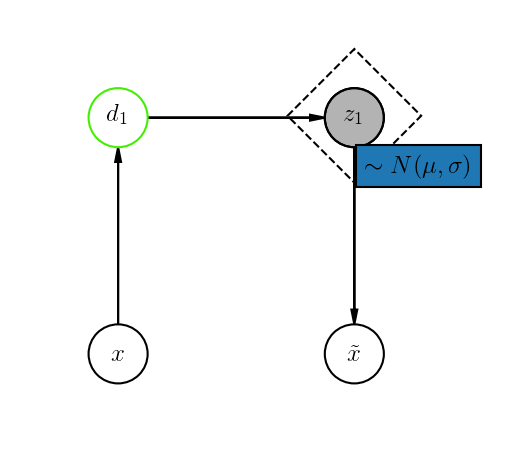
\includegraphics[width=0.33\linewidth]{vae.png}
    \caption{Variational autoencoder}
    \label{fig:vae}
\end{figure}

\vspace{4mm}

\par As we can see in (\ref{fig:vae}) the variational autoencoder is outlined. The general intuition is that a neural network approximates $q_{\phi}(\bm{z} | \bm{x})$ over that dataset and it is assumed that it takes a multivariate Gaussian form for the true, intractable posterior $p_{\vartheta_{real}}(\bm{z} | \bm{x})$.

\vspace{4mm}

\par We sample $\bm{z}$ from a Gaussian where the mean and standard deviation is the output of the probabilistic encoder and than we apply the reparametrization trick. With this method the variational lower bound becomes simple to approximate:

\vspace{4mm}

\begin{equation}
    L_{i} \simeq \frac{1}{2}\sum_{j = 1}^{J}\Big( 1 + \ln(\sigma^{(i)}_{j})^{2} - (\mu^{(i)}_{j})^{2} - (\sigma^{(i)}_{j})^{2} \Big) + \frac{1}{L}\sum_{l=1}^{L}\ln p_{\theta}(\bm{x}^{(i)} | \bm{z}^{(i, l)})
    \label{eq:ELBO}
\end{equation}

\vspace{4mm}

\par Where $\bm{z}^{(i, l)} = \bm{\mu}^{(i)} + \bm{\sigma}^{(i)} \odot \bm{\epsilon}^{(l)}$ where $\bm{\mu}, \bm{\sigma}$ come from $q_{\phi}(\bm{z} | \bm{x})$ and $\bm{\epsilon}$ from $p(\bm{\epsilon}) \sim N(0, 1)$. The first part is the Kullback-Leibler-divergence between a unit Gaussian and $N(\mu^{(i)}, \sigma^{(i)})$ can be analytically calculated and was substituted in \ref{eq:ELBO}.

\vspace{4mm}

\par In practice this means that the KL-divergence can be computed efficiently after the encoding and to speed up the learning process usually $L = 1$ is chosen to not to pass the code through the decoder several times. In the case of continuous pixel values the second part of the ELBO can be approximated with a multivariate Gaussian whereas in case of binary pixel values it becomes a Bernoulli-distribution. 

\vspace{5mm}

\subsection{LVAE}

\vspace{5mm}

\par The ladder variational autoencoder was first introduced in 2016 \cite{sonderby2016ladder} one year after the UNET \cite{ronneberger2015u} architecture which used ladder like parameter sharing across encoding and decoding layers. Using ladder like structures became popular around 2015.

\vspace{4mm}

\par I need to emphasise that the LVAE model only differs from the VAE in the inference model $q_{\phi} (z | x)$ by introducing more stochastic layers to provide better reconstruction results and to learn a more abstract latent representation oft the data. In \cite{sonderby2016ladder} they approximated $p_{\theta_{real}}$ by splitting it up two L layers:

\vspace{4mm}

\begin{equation}
    p_{\theta_{real}}(\bm{z}) =  p_{\theta}(\bm{z}_{L})\prod_{i = 1}^{L - 1}p_{\theta}(\bm{z}_i | \bm{z}_{i+1})
\end{equation}

\vspace{4mm}

\par In practice I added one additional layer to the VAE architecture as they did in the above mentioned article. Here:

\vspace{4mm}

\begin{gather*}
    p_{\theta}(\bm{z}_L) = N(\bm{z}_L  ~ | ~ 0, 1) \quad called\ \epsilon\ previously\\
    p_{\theta}(\bm{z}_i ~ | ~ \bm{z}_{i+1}) = N(\bm{z}_i ~ |  ~ \mu_{p,i}(\bm{z}_{i+1}), \sigma_{p, i}(\bm{z}_{i+1}))
\end{gather*}

\vspace{4mm}

\par Of course, I outlined here the case of continuous variables the case where the dataset is not binarized. 

\vspace{4mm}

\begin{figure}[H]
    \centering
    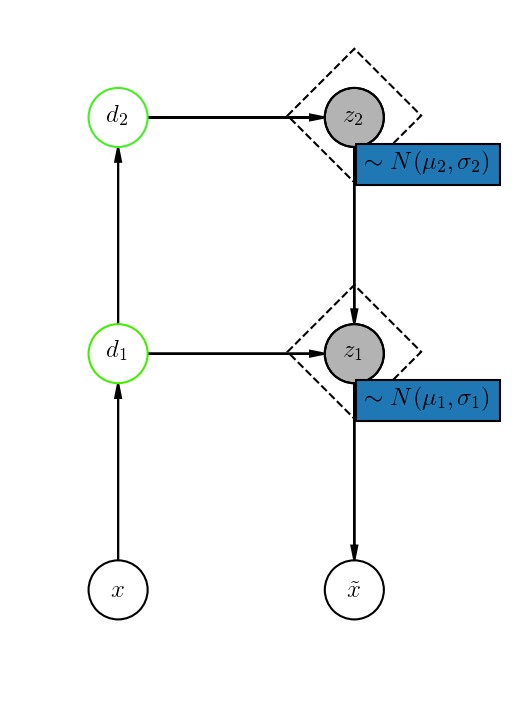
\includegraphics[width=0.35\linewidth]{lvae.png}
    \caption{Ladder variational autoencoder}
\end{figure}

\newpage

\section{Datasets}

\vspace{7mm}

\par Mainly I used synthetically generated texture families with my models that resemble the Simonchelli-Portilla texture family \cite{portilla2003image} but I experimented with the MNIST, Fashion-MNIST \cite{xiao2017fashion}, CIFAR-10, natural textures and the dSprites dataset \cite{matthey2017dsprites}. I wanted to find out whether it would be possible for a latent variable model to disentangle parameters such as contrast from images.

\vspace{4mm}

\par The synthetically generated texture families I used throughout my study contain 7 distinct families. I implemented contrast normalization, the method basically sets the same mean pixel values and same standard deviations between classes, therefore there is no contrast imbalance between different families. By introducing contrast one can see that some features are eliminated or pronounced.

\vspace{4mm}

\begin{figure}[H] 
  \label{fig:texture-families} 
  \begin{minipage}{0.48\linewidth}
    \centering
    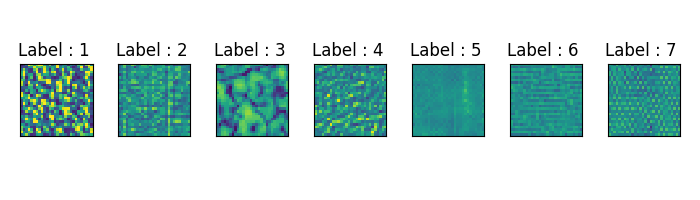
\includegraphics[width=.95\linewidth]{default.png} 
    \caption{Images} 
  \end{minipage}
  \begin{minipage}{0.48\linewidth}
    \centering
    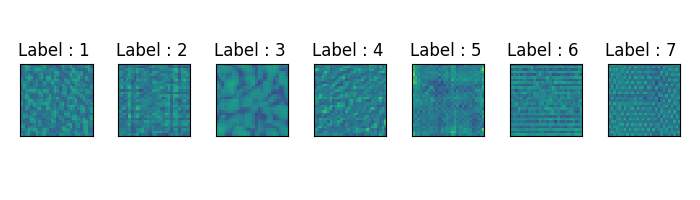
\includegraphics[width=.95\linewidth]{normalized.png} 
    \caption{Normalized images} 
  \end{minipage} 
  
  
  \begin{minipage}{0.48\linewidth}
    \centering
    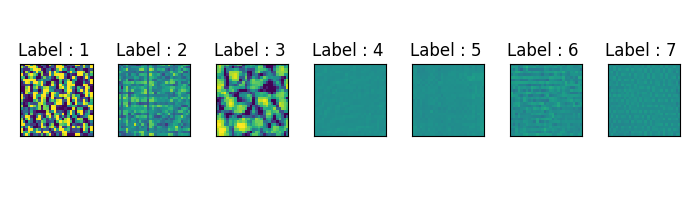
\includegraphics[width=.95\linewidth]{default_contrast.png} 
    \caption{Images - contrast applied} 
  \end{minipage}%% 
  \begin{minipage}{0.48\linewidth}
    \centering
    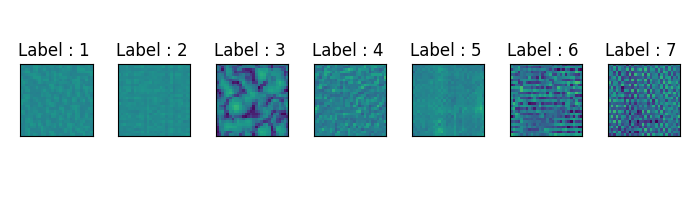
\includegraphics[width=.95\linewidth]{normalized_contrast.png} 
    \caption{Normalized images - contrast applied} 
  \end{minipage} 
\end{figure}

\newpage

\section{Implementation details}

\vspace{7mm}

\par I used the $\beta-$VAE and ($\beta-$)LVAE architectures as I mentioned:

\vspace{4mm}

\begin{equation}
    L_{i} \simeq \beta_{max}\frac{1}{2}\sum_{j = 1}^{J}\Big( 1 + \ln(\sigma^{(i)}_{j})^{2} - (\mu^{(i)}_{j})^{2} - (\sigma^{(i)}_{j})^{2} \Big) + \frac{1}{L}\sum_{l=1}^{L}\ln p_{\theta}(\bm{x}^{(i)} | \bm{z}^{(i, l)})
\end{equation}

\vspace{5mm}

\subsection{Architectural details}

\vspace{5mm}

\par The models were built in Keras \cite{chollet2015keras} and using its built-in visualization tool I was able to show how my modular VAE is constructed:

\vspace{4mm}

\begin{figure}[H]
    \centering
    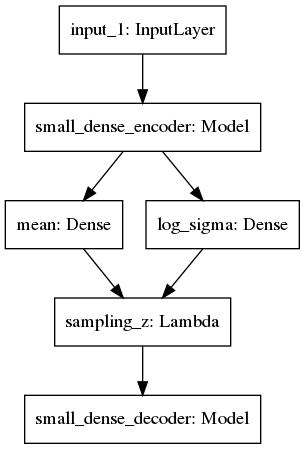
\includegraphics[width=0.25\textwidth]{vae_keras.png}
    \caption{Variational autoencoder implementation in Keras}
\end{figure}

\vspace{4mm}

\par It is a bit confusing since the arrows only mean parameter passes here not dependence as in the graphical representation where the nodes of the graph are random variables as opposed to models. Moving on to the LVAE:

\vspace{4mm}

\begin{figure}[H]
    \centering
    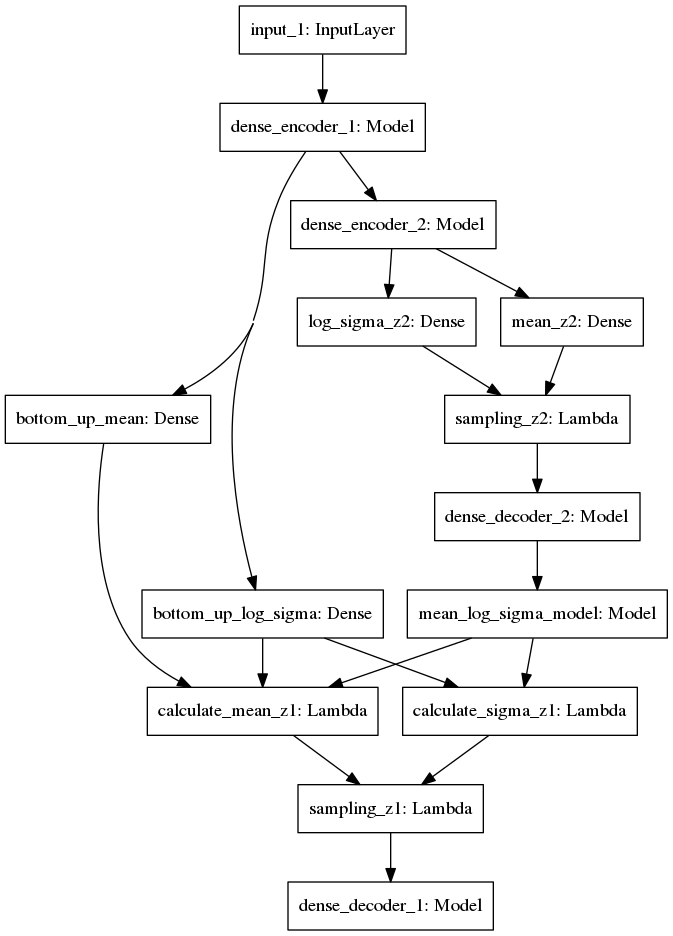
\includegraphics[width=0.6\linewidth]{dense_lvae_keras.png}
    \caption{Ladder variational autoencoder implementation in Keras}
    \label{fig:keras_lvae}
\end{figure}

\vspace{4mm}

\par Keras provides high modularity so the blocks \textit{dense\_encoder\_1, dense\_decoder\_1, etc.} can all be
changed and swapped to higher or lower capacity and complexity modules with MLP \footnote{Multilayer Perceptron} or convolutional architectures.

\vspace{5mm}

\subsection{Incremental $\beta$-learning}

\vspace{5mm}

\par From the original LVAE article \cite{sonderby2016ladder} I used incremental $\beta$ learning, meaning that I raised my $\beta$ value incrementally during learning for 3/7ths of the epochs and kept on learning with $\beta = \beta_{max}$ for the remaining steps. From this article I also tested batch-normalization and built modular models that include convolution with batch-normalization as well. The value $\beta_{max}$ can be set before the start of the training, $\beta_{max} = 1$ is the case of the VAE but raising its value directly emphasizes the influence of the KL-term on the system during training.

\vspace{4mm}

\par For both of my latent variable model architectures (VAE, LVAE) I use the reparametrization trick on the deepest variational parameter to be able to later on sample from a zero centered unit Gaussian:

\vspace{4mm}

\begin{equation}
    \boldsymbol{\bm{z}}^{(i, l)} = \boldsymbol{\mu}^{(i)} + \boldsymbol{\sigma}^{(i)} \odot \boldsymbol{\bm{\epsilon}}^{(l)}
\end{equation}

\vspace{4mm}

\par Where $\boldsymbol{\bm{\epsilon}}^{(l)} \sim \boldsymbol{N}(0, 1)$ in order to be able to achieve that when sampling from the generative model we would only need to sample this $\bm{\epsilon}$ parameter and feed it to the network to generate new samples from the approximated $p_{\vartheta_{real}}(x | z)$ distribution based on the learnt latent representations.

\vspace{5mm}

\subsection{Generative model sampling}

\vspace{5mm}

\par Both models can be sampled after training. However, in the VAE architecture it is straightforward to do so \footnote{generate the random variable and feed it to the decoder}, on the other hand, the LVAE needs bottom up information from the image since the calculation of the mean and standard deviation is deterministic from the generated bottom up (from the input image - referenced as $\bm{bu}$) and top down (from the stochastic latent parameter - referenced as $\bm{td}$) components:

\vspace{4mm}

\begin{gather}
    \label{eq:z1-mean-sigma-1}
    \hat{\sigma}_{1} = \frac{1}{\sigma_{bu}^{-2} + \sigma_{td}^{-2}} \\
    \hat{\mu}_{1} = \frac{\mu_{bu}\sigma_{bu}^{-2} + \mu_{td}\sigma_{td}^{-2}}{\sigma_{bu}^{-2} + \sigma_{td}^{-2}}
    \label{eq:z1-mean-sigma-2}
\end{gather}

\vspace{4mm}

\par When sampling $\bm{z}^{(2)}$, the deepest latent vector, the bottom up standard deviation is considered infinite, therefore:

\vspace{4mm}

\begin{equation}
    \hat{\sigma}_{1} = \sigma_{td}^{2} \quad \quad \hat{\mu_{1}} = \mu_{td}
    \label{eq:ladder-vae-sampling}
\end{equation}

\vspace{4mm}

\par This provides a good way of examining the trained models. Doing a full reconstruction and comparing the bottom up means and standard deviations with the top down means and standard deviations we can find out which of these have a bigger influence on the reconstruction. It might be that we only add noise to the generated images with the stochasticity from the deepest latent variable and only the bottom up components are used for reconstruction, I explore this more in a later section.

\vspace{4mm}

\par My implementation consists mostly dense layers and rectified linear units. Basically each unit of the two-unit ladder encoder includes an MLP in the LVAE architecture. Also, I experimented with convolutional and deconvolutional \footnote{referred to also as transpose convolution, inverse convolution} encoders and decoders for both the VAE and LVAE architectures. However, deconvolution usually results in pixelated images with a checkered pattern, in order to compensate this, I replaced it with bilinear upsampling and convolution \cite{odena2016deconvolution}. Not only did I create variational/stochastic models but also I implemented autoencoders with no restriction on the latent space for comparison.

\vspace{4mm}

\par In (\ref{fig:vae}), (\ref{fig:keras_lvae}) it can be spotted that there is an intermediate step included in the generation process of the standard deviations. Since linear layers are constructing the means and the standard deviations they are not restricted to be positive which is not an issue for the means of Gaussian distributions but for the standard deviations. It is usually resolved as generating the logarithm of the standard deviations and then taking their exponential each time their value is needed.

\vspace{5mm}

\subsection{Tools and resources}

\vspace{5mm}

\par As I mentioned during the description of the models used, I implemented everything in the framework Keras and also heavily relied on the package $\bm{tensorflow\_probability}$ to be able to include statistical methods, such as probability distribution sampling in my code. In addition, I want to emphasize that I have build a Python library out of my code to provide a framework to test variational autoencoders with different datasets. The package is available via $\bm{pip}$ \footnote{\url{https://pypi.org/project/csnl-vae-olaralex/}} and the corresponding datasets to use with some example Jupyter notebooks are available through Kaggle \footnote{\url{https://www.kaggle.com/dumbo666/wigner-csnl-textures-mnist-format}}.

\newpage

\section{Methods and goals}

\vspace{7mm}

\subsection{Disentangling contrast}

\vspace{5mm}

\par I wanted to encode high level information in the latent code. In order to do so I implemented some random contrast factor on the training data while feeding it through my networks in batches. This mode could have been switched on and off by a function flag to apply additional contrast or not. All my datasets contained continuous values in the range $[0, 1]$. I applied the following non-deterministic function on each image of a batch:

\vspace{4mm}

\begin{equation}
    \Tilde{I}(x, y) = clip\Big(R \cdot [I(x, y) - 0.5] + 0.5\Big)_{\ [0, 1]}
\end{equation}

\vspace{4mm}

\par Where $I(x, y)$ is the original image, I approximated the global mean with $0.5$ therefore the multiplication by the random number $R$ for each image directly modified the standard deviation of the image, therefore its global contrast.

\vspace{4mm}

\par With this method I wanted to encode a variable in the latent code that can directly disentangle contrast from images. This has been done with a factorized prior and researchers at Google had an immense success with it \cite{DBLP:journals/corr/abs-1811-12359}. My attempt here is to build a hierarchical model without the factorized restriction that resembles the visual cortex and exhibits almost disentangled behaviour in one or more hidden units.

\vspace{5mm}

\subsection{Incremental $\beta$-learning}

\vspace{5mm}

\par By incrementally changing the coefficient of the KL-term of the joint loss function in \cite{sonderby2016ladder} it is stated that - as they call it - warm-up results in more active units therefore a more distributed latent representation is achieved. I measure this in the results section when I compare correlations of latent code with random contrast values applied to images.

\vspace{4mm}

\par It can be heuristically explained why warm-up/incremental $\beta$-learning helps the process. Since with $\beta = 0$ the VAE becomes similar to simple auto-encoder, for which the primary goal is to reconstruct the given examples perfectly, we incrementally add the restriction to the latent space, therefore a better reconstruction is achieved with not randomly initialized weights by the time that the KL-term influences the latent space significantly. I examine the case where $\beta_{max}$ is high and therefore has a substantial influence on reconstruction quality and latent structure.

\vspace{5mm}

\subsection{Statistical analysis}

\vspace{5mm}

\par After training a model for several epochs we have an inference model which is not very interesting. Since in best conditions it reconstructs the images provided to it perfectly. We want to be able to sample from $p_{\bm{\epsilon}}$, pass the sampled value through the decoder and achieve previously unseen but visually pleasing images of the same sort as the used dataset. For this we use the generative or decoder model. 

\vspace{4mm}

\par In order to do this I implemented several sampling processes. One samples the prior distribution $N x N$ times where $N$ is a function parameter and plots the results on a grid. This shows whether the latent space became meaningful at all. I also implemented sweeping in the latent space where each component of the latent code can be chosen and by sampling from $p(\bm{\epsilon})$ once an changing only $\epsilon_{i}$ in a range one can visualize what each latent component does. Since they are not completely independent this method only provides an intuition, however, when combined with contrast one can hope to find parameters which mostly encode that.

\vspace{4mm}

\begin{figure}[ht] 
  \begin{minipage}{0.48\linewidth}
    \centering
    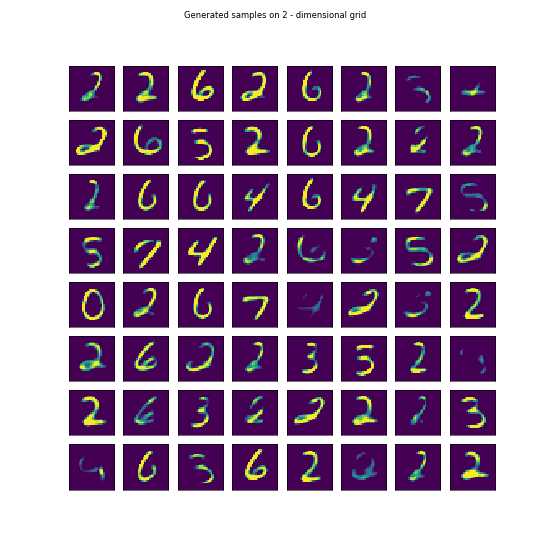
\includegraphics[width=.65\linewidth]{gen/generated_samples_mnist_dense_vae.png}
    \caption{Sampled images from a trained generative model on the MNIST dataset with dense encoder/decoder and $\beta$-VAE architecture}
    \label{fig:sampled-images-1}
  \end{minipage}\hfill
  \begin{minipage}{0.48\linewidth}
    \centering
    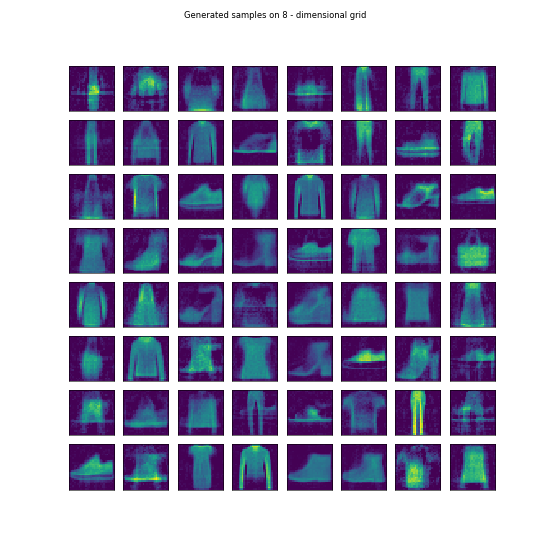
\includegraphics[width=.65\linewidth]{gen/generated_samples_fashion_mnist_dense_vae.png} 
    \caption{Sampled images from a trained generative model on the FashionMNIST dataset with dense encoder/decoder and $\beta$-VAE architecture} 
    \label{fig:sampled-images-2}
  \end{minipage} 
\end{figure}

\vspace{4mm}

\par But how can the contrast component be found in the latent code? In order to answer this question I implemented correlation analysis of latent codes. In the case of the VAE architecture I only correlated the latent code with the random contrast values that I applied to images. In the case of the LVAE architecture I did this for both stochastic set of units. However, this is not enough to find out the sweeping range but the component index that encodes contrast. I also analyzed the average value of hidden units and their standard deviation in order to shed light on these things.

\vspace{4mm}

\subsection{Label correlation anaylisis}

\vspace{4mm}

\par For labeled data (MNIST, FashionMNIST, textures) I could also correlate the one hot encoded labels with the latent code for each class. With this method I could measure which latent components reacts to which class labels mostly. By changing its value I wanted to find out whether the texture-family or the corresponding digit features can be suppressed or not.

\vspace{4mm}

\begin{figure}[H]
    \centering
    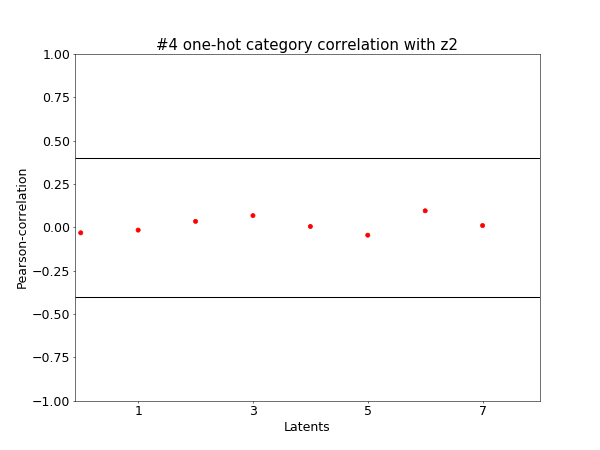
\includegraphics[width=0.55\textwidth]{17_DenseLinLinLadderVAE_contrastNorm-cat-4-to-z2-corr.png}
    \caption{Linear + dense encoders and dense + linear decoders LVAE architecture with contrast normalization, showing the $4$th category pairwise correlation for a large, representative batch with $\bm{z^{(2)}}$}
\end{figure}

\vspace{4mm}

\par For the LVAE architecture, there are two different levels where stochastic sampling is implemented. The deepest latent is sampled from our prior but the intermediate layer that contains bottom up information during training from the input image, and top down information from the deepest latent space contains crucial information during latent vector sampling. I already mentioned this previously but it is crucial to examine whether the top down information is used at all or resembles the resulting mean and standard deviations. As it can be the case that during training only the first latent layer is used, that deepest layer only adds noise but the capacity of the models results in good reconstructions. However, the goal here is not pristine reconstruction quality but representational learning. I implemented histogram analysis of vector values both for the means and standard deviations during a full reconstruction through the system. I also implemented visualizations to actually see how similar these vectors are with diverging colors for the vector values.

\vspace{4mm}

\begin{figure}[H]
    \centering
    
\includegraphics[width=0.3\textwidth]{diverging_color.png}
    \label{fig:diverging_colors}
    \caption{Diverging colors used for latent code visualization}
\end{figure}

\vspace{4mm}

\subsection{UMAP decomposition}

\vspace{4mm}

\par I also experimented with UMAP \cite{mcinnes2018umap} and  t-SNE \cite{maaten2008visualizing} embeddings on the latent code(s) and reconstructed data to see whether the image/texture classes are decomposed in the embedding space. It is also crucial to see whether in the case of the LVAE if $\bm{z}^{(2)}$ contains more, less or the same information as $\bm{z}^{(1)}$. This question is motivated by the fact that in \cite{ZiembaV2} they suggest that the V2 codes different information as the V1 and hierarchical models use different information in different levels in the mammalian brain from the same input. For computational efficiency I used UMAP since it is significantly faster and produces visually similar results to t-SNE.

\begin{figure}[H] 
  \begin{minipage}{0.48\linewidth}
    \centering
    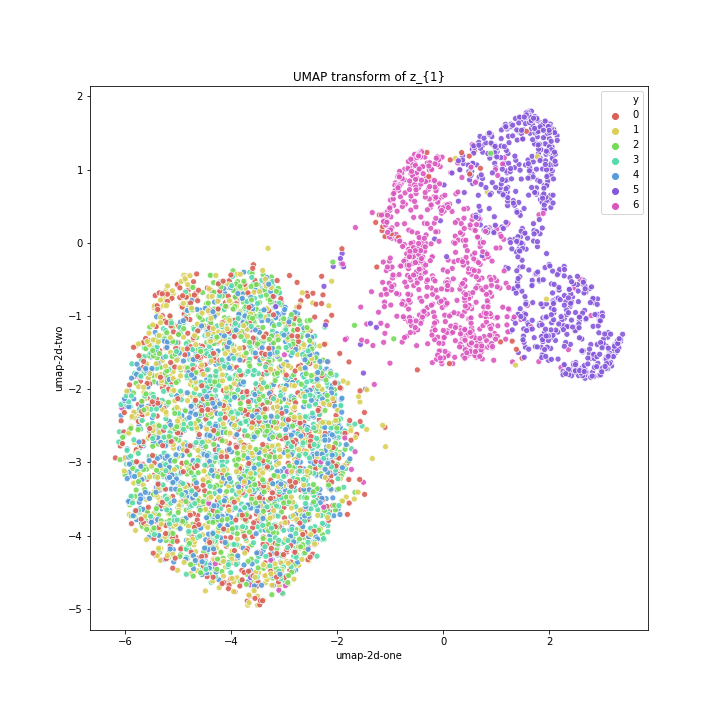
\includegraphics[width=.7\linewidth]{umap_z1_dense_lin_lin_no_norm.png}
    \caption{UMAP decomposition of $\bm{z^{(1)}}$ from a trained LVAE architecture with linear + dense encoders and dense + linear decoders}
    \label{fig:umap-z1}
  \end{minipage}\hfill
  \begin{minipage}{0.48\linewidth}
    \centering
    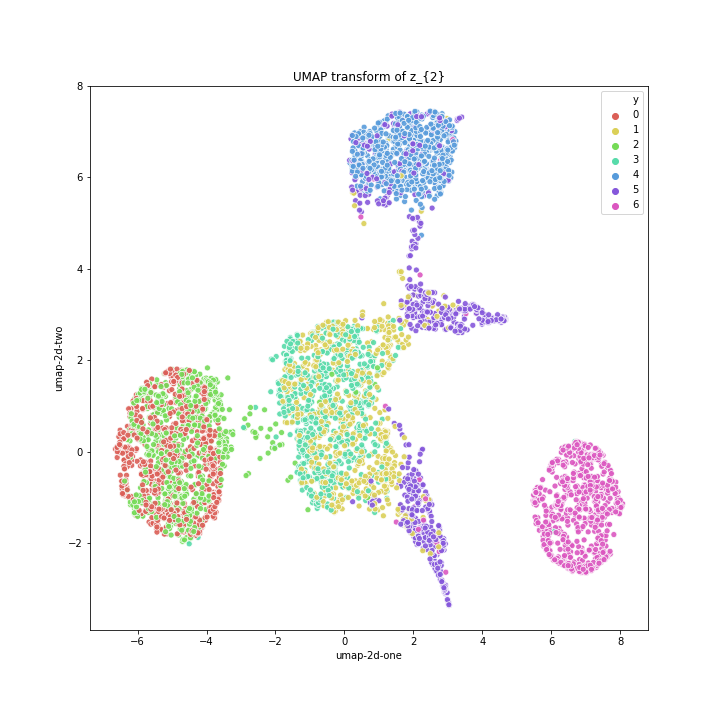
\includegraphics[width=.7\linewidth]{umap_z2_dense_lin_lin_no_norm.png} 
    \caption{UMAP decomposition of $\bm{z^{(2)}}$ from a trained LVAE architecture with linear + dense encoders and dense + linear decoders} 
    \label{fig:umap-z2}
  \end{minipage} 
\end{figure}

\vspace{4mm}

\par With the same decomposition I present here the corresponding textures not just their labels what we can notice in the following figures is that the UMAP embedding suggests that some information is lost and some information is gained from $\bm{z}^{(1)}$ to $\bm{z}^{(2)}$, since in (\ref{fig:umap-z1}, \ref{fig:umap-z1-text}) categories $5$, $6$ are properly separated into two distinct groups while label $5$ is separated into 3 folds in (\ref{fig:umap-z2}, \ref{fig:umap-z2-text}) and is even mixing with $3$. On the other hand, two mixed groups are separated in the deepest latent code.

\vspace{4mm}

\begin{figure}[H] 
  \begin{minipage}{0.48\linewidth}
    \centering
    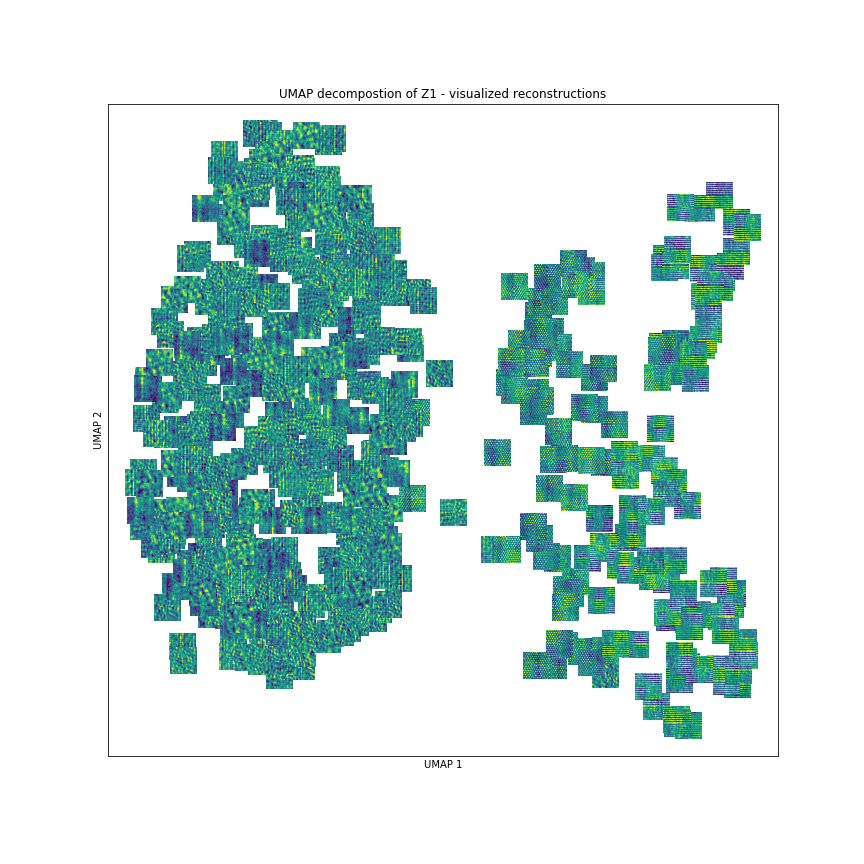
\includegraphics[width=.7\linewidth]{umap_z1_dense_lin_lin_no_norm_textures.png}
    \caption{UMAP decomposition of $\bm{z^{(1)}}$ from a trained LVAE architecture with linear + dense encoders and dense + linear decoders, each point is represented with the reconstruction from the corresponding texture family}
    \label{fig:umap-z1-text}
  \end{minipage}\hfill
  \begin{minipage}{0.48\linewidth}
    \centering
    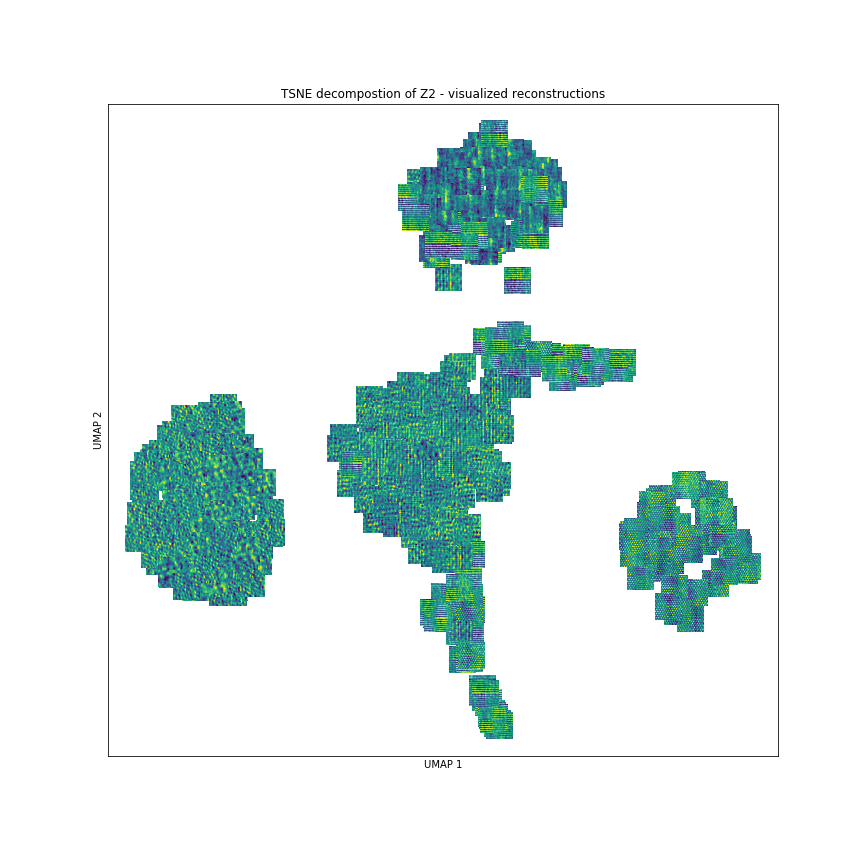
\includegraphics[width=.7\linewidth]{umap_z2_dense_lin_lin_no_norm_textures.png} 
    \caption{UMAP decomposition of $\bm{z^{(2)}}$ from a trained LVAE architecture with linear + dense encoders and dense + linear decoders, each point is represented with the reconstruction from the corresponding texture family} 
    \label{fig:umap-z2-text}
  \end{minipage} 
\end{figure}

\vspace{4mm}

\par We also measured pairwise linear correlation - Pearson-correlation - between $\bm{z}^{(1)}$ and $\bm{z}^{(2)}$.

\vspace{4mm}

\begin{figure}[H]
    \centering
    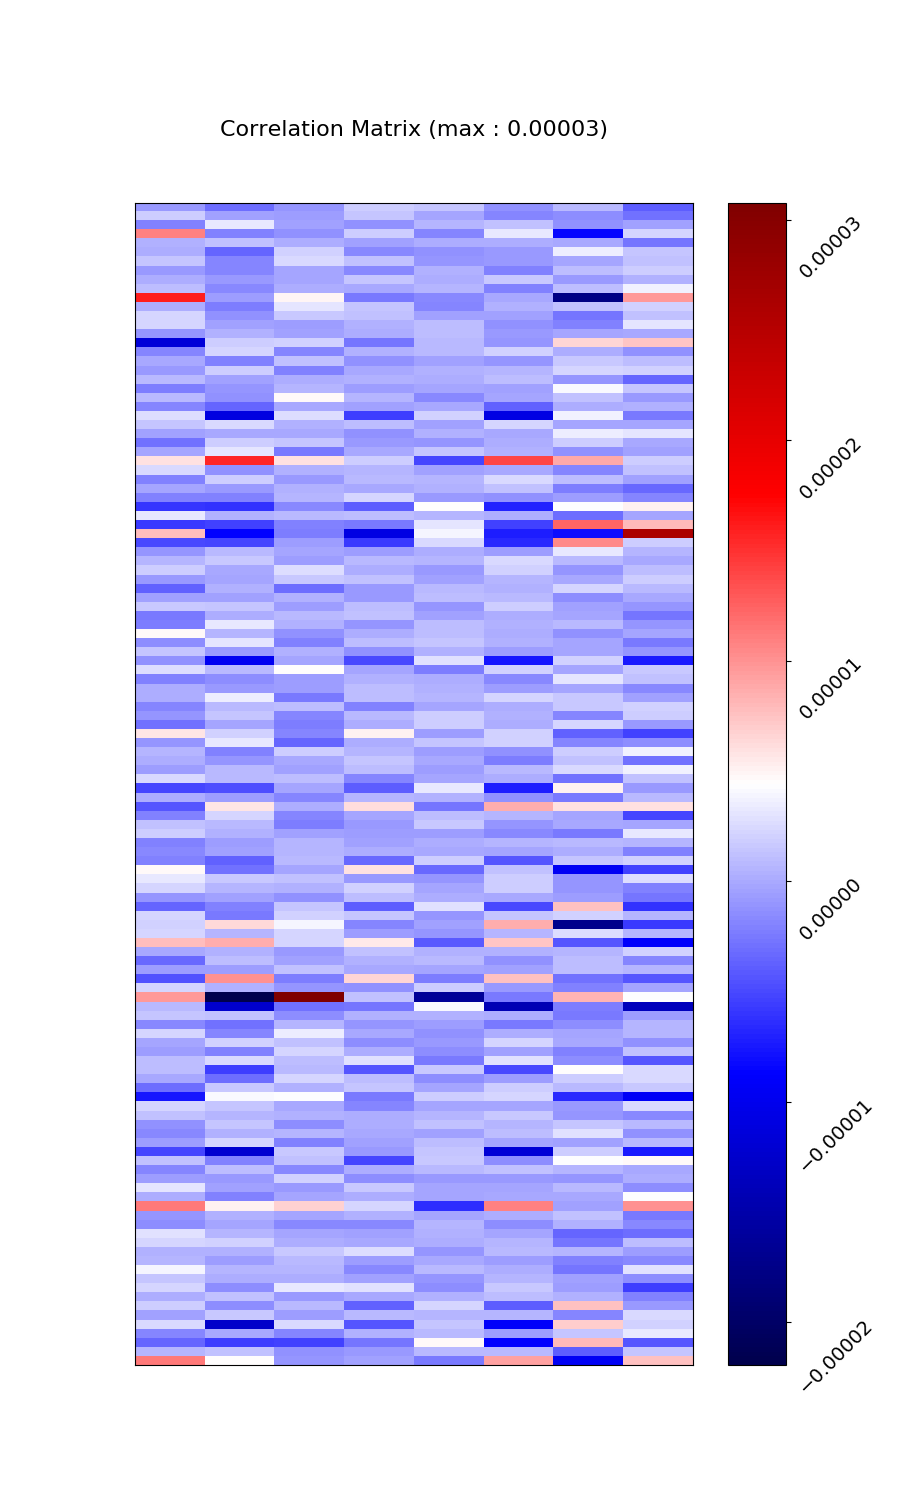
\includegraphics[width=0.3\textwidth]{z1_z2_correlation.png}
    \label{fig:pearson-matrix}
    \caption{Pearson-correlation between $\bm{z}^{(1)}$ and $\bm{z}^{(2)}$}
\end{figure}

\newpage

\section{Results}

\vspace{7mm}

\subsection{Auto-Encoders}

\vspace{5mm}

\par Auto-encoders are not generative models but non-linear functions that are learning to reconstruct unlabelled data by pushing it through a usually reduced dimensionality gate. This low-dimensional representation with the decoder architecture can be ported to everywhere and for large datasets it can save much more space than regular compression tools such as JPEG, JPEG-2000. It is important to mention that compression via auto-encoders is highly dataset specific so it cannot be used as conveniently as JPEG without training a neural network. Also, the compression is lossy so the images cannot be fully reconstructed without some information loss.

\vspace{4mm}

\par Results are presented using the well-known MNIST dataset with binarized values and Bernoulli-loss:

\vspace{4mm}

\begin{figure}[H] 
  \label{fig:auto_encoder_results} 
  \begin{minipage}{0.48\linewidth}
    \centering
    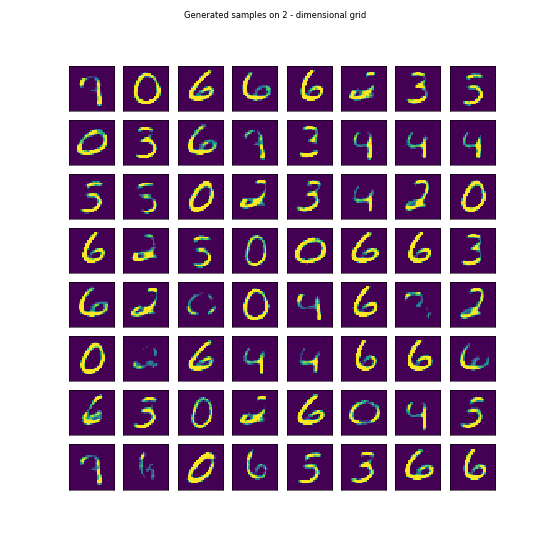
\includegraphics[width=.65\linewidth]{gen/generated_samples_mnist_auto_encoder.png} 
    \caption{Sampled images} 
  \end{minipage}\hfill
  \begin{minipage}{0.48\linewidth}
    \centering
    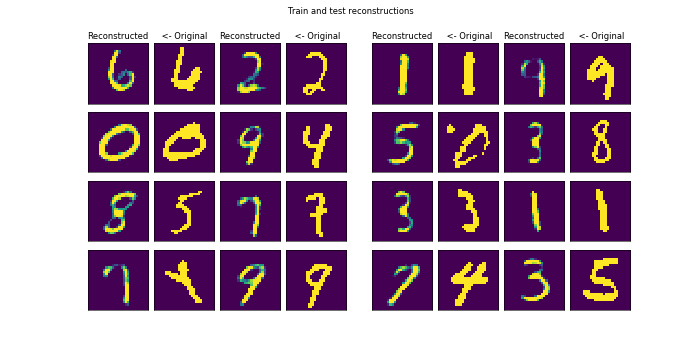
\includegraphics[width=.95\linewidth]{reco/reconstrunction_samples_mnist_auto_encoder.png} 
    \caption{Reconstructed images} 
  \end{minipage} 
\end{figure}

\vspace{4mm}

\par The latent representation contained length two vectors and it can be seen that such low complexity data is well represented even without constraint on the code.

\newpage

\subsection{Variational auto-encoders}

\vspace{5mm}

\par Results are presented using the Fashion-MNIST dataset with continuous values in $[0, 1]$ and normal loss:

\vspace{4mm}

\begin{figure}[ht] 
  \label{fig:auto_encoder_results} 
  \begin{minipage}{0.5\linewidth}
    \centering
    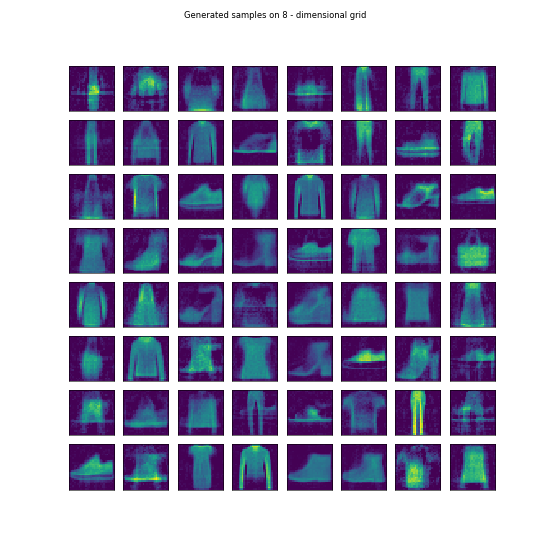
\includegraphics[width=.65\linewidth]{gen/generated_samples_fashion_mnist_dense_vae.png} 
    \caption{Sampled images} 
  \end{minipage}%%
  \begin{minipage}{0.5\linewidth}
    \centering
    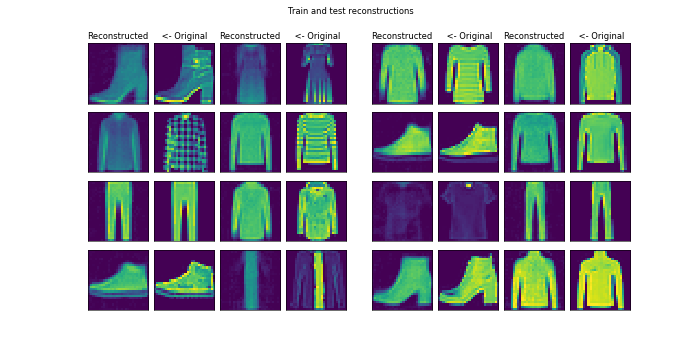
\includegraphics[width=.95\linewidth]{reco/reconstrunction_samples_fashion_mnist_dense_vae.png} 
    \caption{Reconstructed images} 
  \end{minipage} 
\end{figure}

\vspace{4mm}

\par The latent representation contained length eight vectors and it was trained with $\beta = 1$.

\vspace{4mm}

\par Using the same eight piece code and the same training iterations, the effect of the variational inference can be seen in the latent representation compared to the non-variational model:

\begin{figure}[ht] 
  \label{fig:auto_encoder_results} 
  \begin{minipage}{0.5\linewidth}
    \centering
    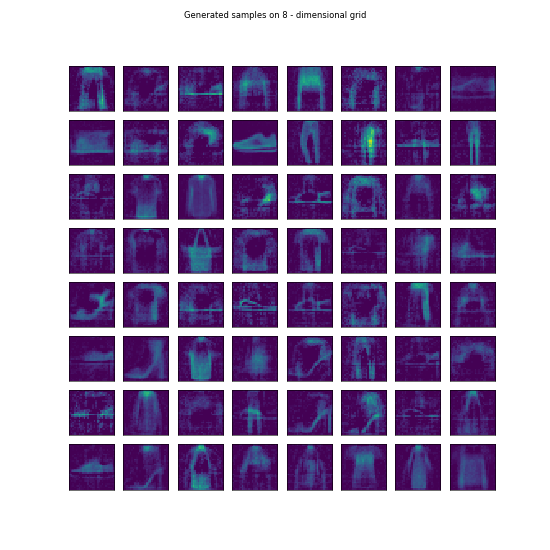
\includegraphics[width=.65\linewidth]{gen/generated_samples_fashion_mnist_auto_encoder.png} 
    \caption{Sampled images} 
  \end{minipage}%%
  \begin{minipage}{0.5\linewidth}
    \centering
    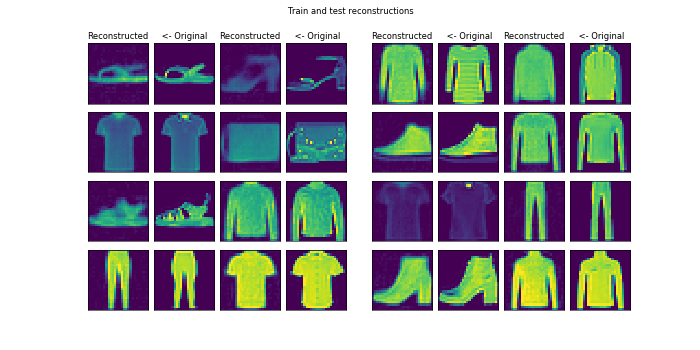
\includegraphics[width=.95\linewidth]{reco/reconstrunction_samples_fashion_mnist_auto_encoder.png} 
    \caption{Reconstructed images} 
  \end{minipage} 
\end{figure}

\vspace{4mm}

\par In the reconstructions the effect cannot be seen but it is easily observed in the latent representation since it is less pronounced in the non-variational model.

\newpage

\subsection{Ladder variational auto-encoders}

\vspace{5mm}

\par The ladder architecture introduces an additional layer of abstraction into our variational model. Better latent representations are expected using this as our model.

\vspace{4mm}

\par Training a deeper model poses difficulties since training it efficiently is much harder and usually many more iterations are needed. Since randomly initialized weights might provide a very bad spot on the loss landscape the deviation in the KL-term can be very high and latent representations are basically non-existent. The connection between the bottom up and top down components at the intermediate layer also poses a threat since information sharing provides a loophole to the model not to abstract information and just leave the deeper stochastic code out of the process. 

\vspace{4mm}

\par This effect can be handled in a few different ways such as: restricting the encoders first layer to be linear and the decoder at the top to be linear as well, this results in forcing the models to use deeper layers since a very low level of abstraction can be achieved with such low complexity models. A higher $\beta_{max}$ can achieve similar effect since the KL-term can influence the overall loss more and could also force the model to use deeper representations in order to lower the KL-loss significantly. 

\vspace{4mm}

\par In the following sections I mostly used different architectures of LVAEs with constrained linear encoders and decoders, with dense and convolutional encoders and decoders as well.

\vspace{7mm}

\subsection{Understanding disentangled representations of contrast}

\vspace{5mm}

\par As I mentioned previous I implemented random contrast learning, meaning that some random amount of contrast is added to the input images to make the model contrast independent by disentangling the contrast in the latent code. I looked into what is necessary in order to acquire such disentangled representation.

\vspace{4mm}

\par Here I present some results with linear modules at the first encoder and last decoder layer with and without contrast normalization with the same settings: $[\bm{z}_{1}] = 128, [\bm{z}_{2}] = 8$:

\vspace{4mm}

\begin{figure}[H] 
  \begin{minipage}{0.5\linewidth}
    \centering
    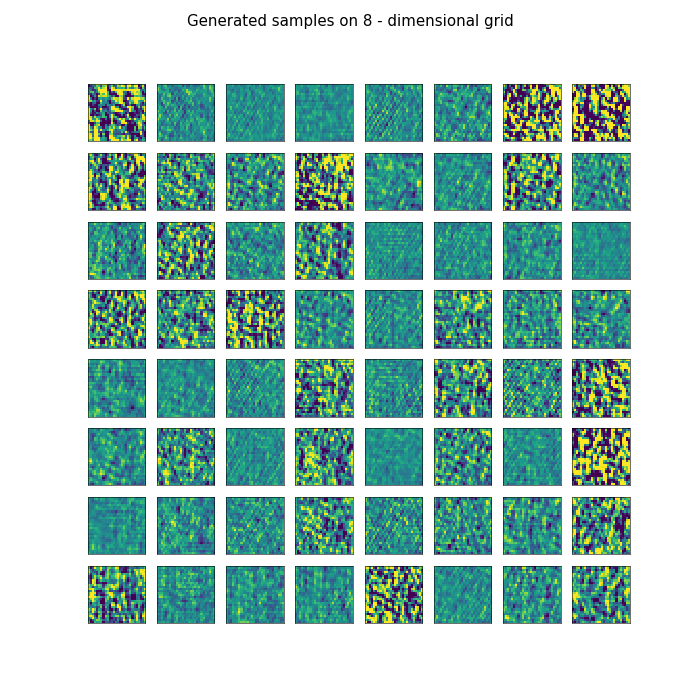
\includegraphics[width=.75\linewidth]{contrast/generated_samples_noContrastNorm_noContrast.png} 
    \caption{No contrast - no normalization} 
    \label{fig:contrast-generated-1} 
  \end{minipage}%%
  \begin{minipage}{0.5\linewidth}
    \centering
    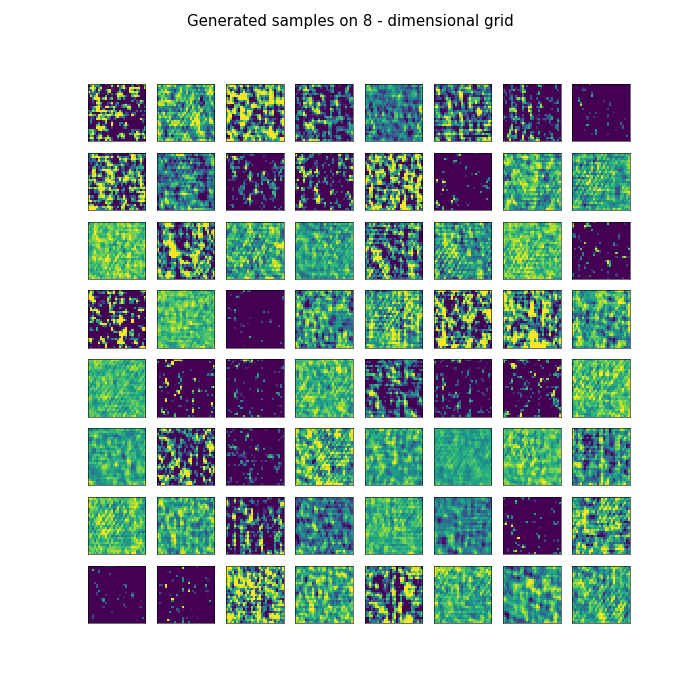
\includegraphics[width=.75\linewidth]{contrast/generated_samples_noContrastNorm_contrast.png} 
    \caption{Contrast - no normalization} 
    \label{fig:contrast-generated-2} 
  \end{minipage} 
  \begin{minipage}{0.5\linewidth}
    \centering
    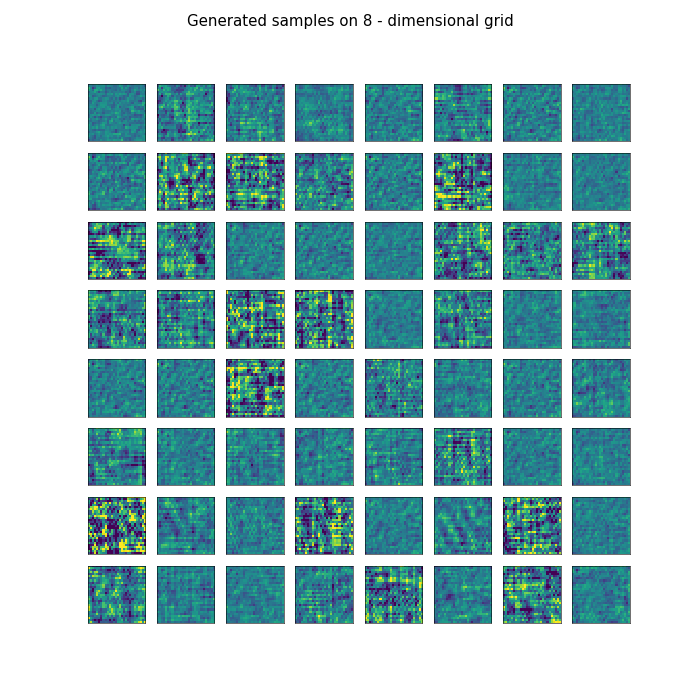
\includegraphics[width=.75\linewidth]{contrast/generated_samples_contrastNorm_noContrast.png} 
    \caption{No contrast - normalization} 
    \label{fig:contrast-generated-3} 
  \end{minipage}%% 
  \begin{minipage}{0.5\linewidth}
    \centering
    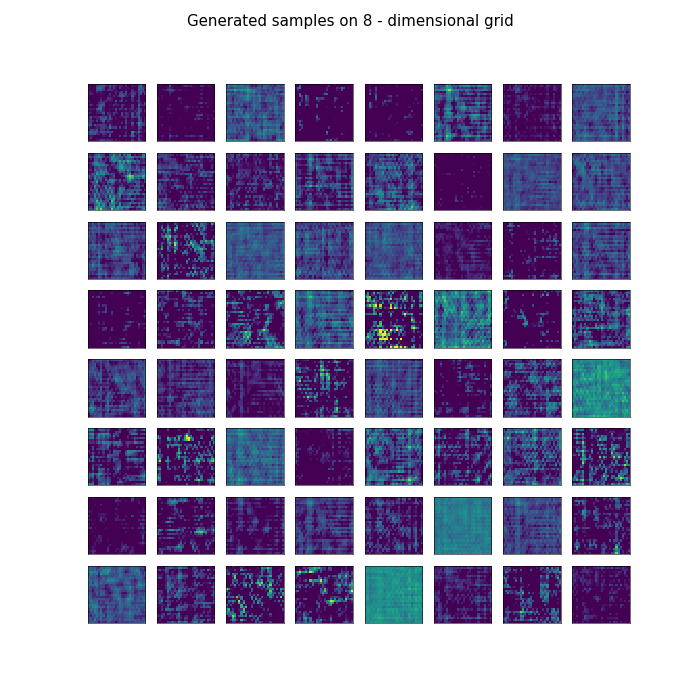
\includegraphics[width=.75\linewidth]{contrast/generated_samples_contrastNorm_contrast.png} 
    \caption{Contrast - normalization} 
    \label{fig:contrast-generated-4} 
  \end{minipage} 
\end{figure}

\vspace{4mm}

\par What we can see in (\ref{fig:contrast-generated-1}, \ref{fig:contrast-generated-2}, \ref{fig:contrast-generated-3},\ref{fig:contrast-generated-4}) is not trivial to compare, however, just by looking at them we can see how contrast modifies training, since we can observe large variance in contrast amongst the generated textures and also normalization can be observed in contrast of images.

\vspace{4mm}

\par A more thorough and systematic comparison can be gained by comparing contrast correlation with the latent codes. This can be done by generating random contrast values. Assuming a batch size $B_{s}$ and latent code dimension $d$ we can correlate the latent code at index $i$ of each element in the batch $z^{(i)}_{\{j\}_{j = 1}^{B_{s}}}$ with the random contrast values of the batch. Calculating simple Pearson-correlation:

\vspace{4mm}

\begin{equation*}
    \rho(\bm{z}^{(i)}, \bm{R_{c}}) = \frac{Cov(\bm{z}^{(i)}, \bm{R_{c}})}{\sigma(\bm{z}^{(i)})\sigma(\bm{R_{c}})}  
\end{equation*}

\vspace{4mm}

\par In this form both the random contrast $\bm{R_{c}}$ and the $i$th component of the latent code for each element in the batch $\bm{z}^{(i)}$ have size $B_{s}$, so comparing these for each of the contrast-normalization models:

\vspace{4mm}

\begin{figure}[H] 
  \label{fig:contrast-correlation} 
  \begin{minipage}{0.5\linewidth}
    \centering
    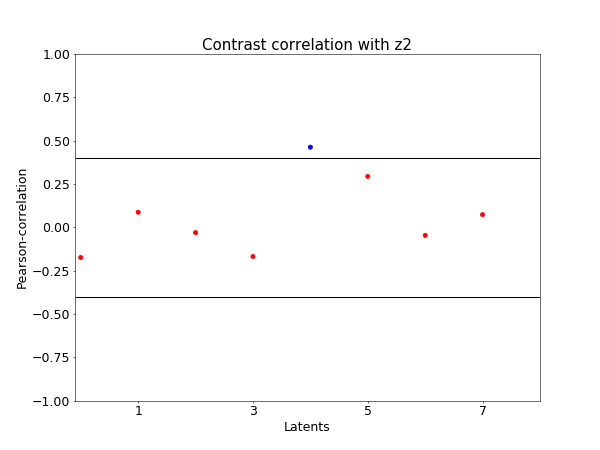
\includegraphics[width=.72\linewidth]{contrast_to_latent/no_norm_contrast_z2_corr.png} 
    \caption{No contrast - no normalization} 
    \label{fig:no-contrast-no-norm}
  \end{minipage}%%
  \begin{minipage}{0.5\linewidth}
    \centering
    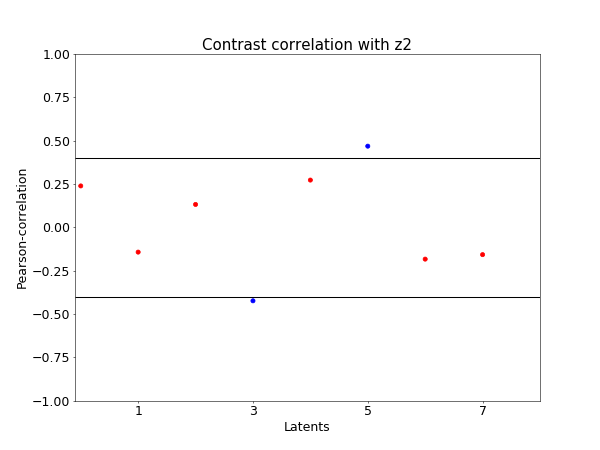
\includegraphics[width=.72\linewidth]{contrast_to_latent/no_norm_contrast_contrast_z2_corr.png} 
    \caption{Contrast - no normalization} 
    \label{fig:contrast-no-norm}
  \end{minipage} 
  \begin{minipage}{0.5\linewidth}
    \centering
    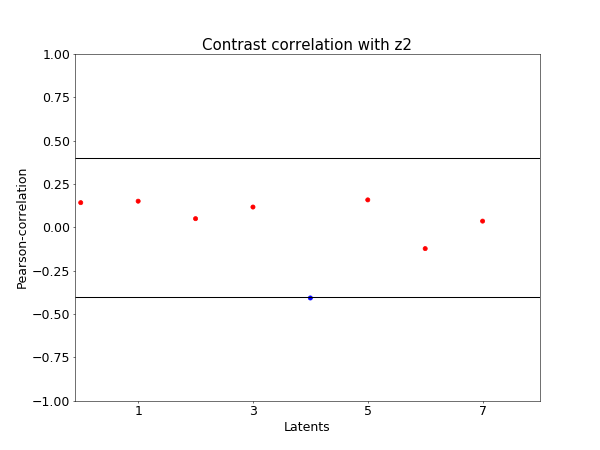
\includegraphics[width=.72\linewidth]{contrast_to_latent/norm_no_contrast_correlation.png} 
    \caption{No contrast - normalization} 
    \label{fig:no-contrast-norm}
  \end{minipage}%% 
  \begin{minipage}{0.5\linewidth}
    \centering
    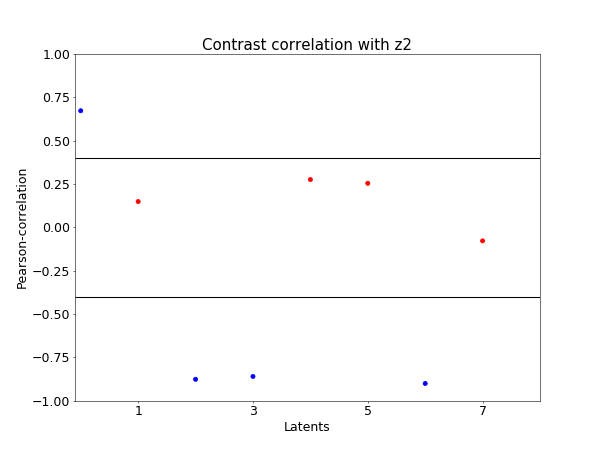
\includegraphics[width=.72\linewidth]{contrast_to_latent/norm_contrast_correlation.png} 
    \caption{Contrast - normalization} 
    \label{fig:contrast-norm}
  \end{minipage} 
\end{figure}

\vspace{4mm}

\par Here we can see that in (\ref{fig:no-contrast-no-norm}) there seems to be natural contrast in this type of dataset and it seems to be disentangled in the $4$th latent code component \footnote{indexing from $0$}. I'll also analyze whether this is the case or the latent code represents a class that has high variability in contrast and only disentangles that class. Adding additional contrast (\ref{fig:contrast-no-norm}) to the textures made two variables to encode something like contrast.

\vspace{4mm}

\par The case is very similar with contrast normalization (\ref{fig:no-contrast-norm}, \ref{fig:contrast-norm}) although this is not expected. This could mean that contrast normalization failed or that the parameter that is seemingly encodes contrast \footnote{has high correlation with what we call contrast} actually encodes a class that has high variability locally even though it was globally normalized.

\vspace{4mm}

\par Observing the labels and their correlation with the deepest latent code $\bm{z}_{2}$ I found that the correlation in each variable with respect to the contrast or the one-hot-encoded $1$st label is almost the same in the non normalized setting:

\vspace{4mm}

\begin{figure}[H]
\begin{minipage}{0.5\linewidth}
    \centering
    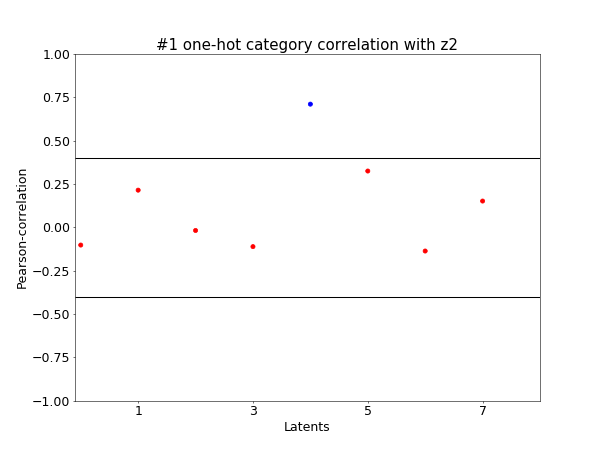
\includegraphics[width=.72\linewidth]{label-contrast-corr/cat-1-to-z2-corr.png} 
    \caption{$1$st one-hot encoded label to $\bm{z}_{2}$} 
    \label{fig:label-contrast-corr-1}
\end{minipage}%% 
\begin{minipage}{0.5\linewidth}
    \centering
    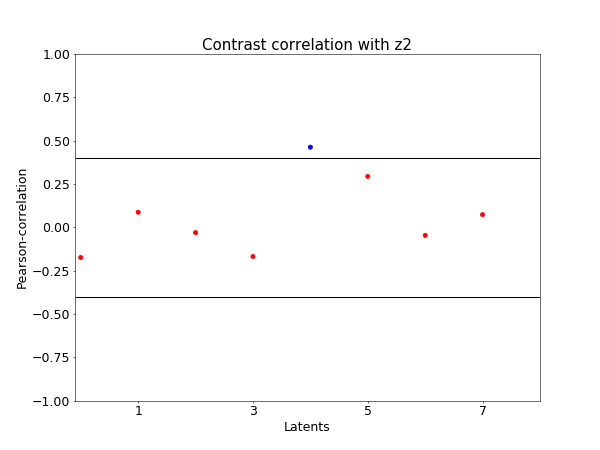
\includegraphics[width=.72\linewidth]{label-contrast-corr/contrast-to-z2-corr.png} 
    \caption{Contrast to $\bm{z}_{2}$} 
    \label{fig:label-contrast-corr-2}
\end{minipage} 
\end{figure}

\par With the non-normalized setting when there is additional contrast there are also high correlations with some of the one-hot-encoded labels therefore no clean disentanglement is provided by the latent representation.

\vspace{4mm}

\par However, another observation can be made by checking that normalized setting. In this scenario the label correlations with $\bm{z}_{2}$ are negligible in both cases of no contrast and additional contrast during training. This leads me to believe that the parameter that correlates with the additional contrast during reconstruction is encoding the local contrast in the normalized scenario. To test this I mentioned earlier that I implemented latent sweep in my code base. Also I made sure that I the latent codes are used in the trained models by observing there means and standard deviations during reconstruction, if these are different from zero and one respectively, meaning that they are not unit Gaussians but some kind of learnt posteriors the models are actually using them for something.

\vspace{4mm}

\begin{figure}[H] 
  \label{fig:contrast-correlation} 
  \begin{minipage}{0.33\linewidth}
    \centering
    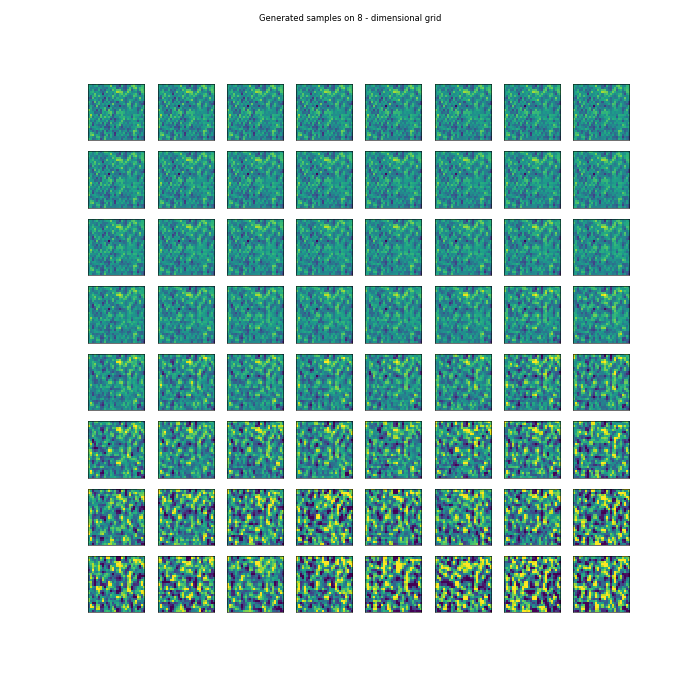
\includegraphics[width=.72\linewidth]{sweep/no_norm_no_contrast_sweep_minus_two_to_one.png} 
    \caption{No contrast, no \newline norm. sweep in $[-2, 1]$} 
    \label{fig:no-contrast-no-norm-sweep}
  \end{minipage}%%
  \begin{minipage}{0.33\linewidth}
    \centering
    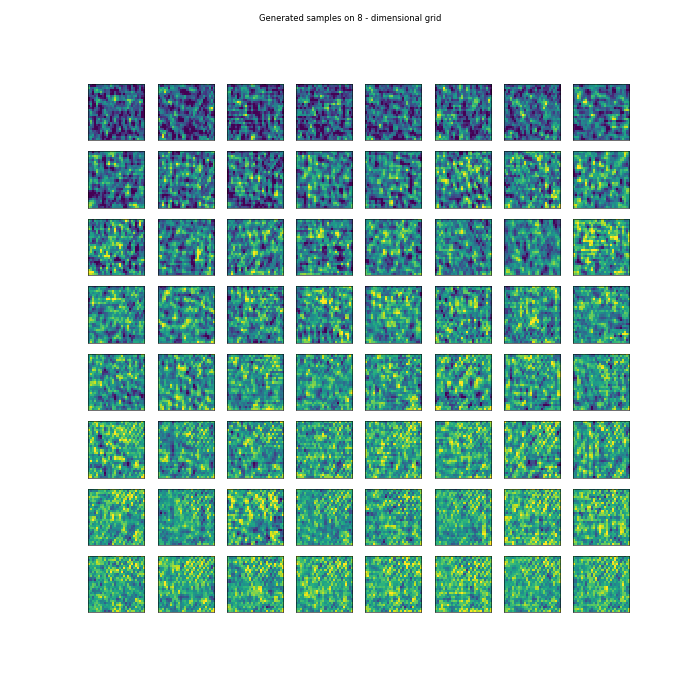
\includegraphics[width=.72\linewidth]{sweep/no_norm_contrast_sweep_minus_two_to_two_3rd_param.png} 
    \caption{Contrast, no norm. \newline sweep in $[-2, 2]$ $3$rd component} 
    \label{fig:contrast-no-norm-sweep-3}
  \end{minipage} 
  \begin{minipage}{0.33\linewidth}
    \centering
    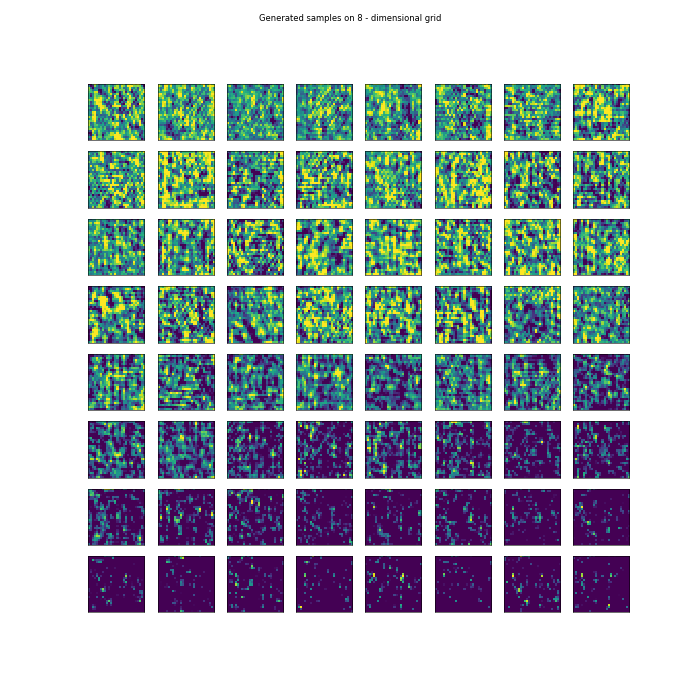
\includegraphics[width=.72\linewidth]{sweep/no_norm_contrast_sweep_minus_two_to_two_5th_param.png} 
    \caption{Contrast, no norm. \newline sweep in $[-2, 2]$ $5$th component} 
    \label{fig:contrast-no-norm-sweep-5}
  \end{minipage}
  %% stats
  \begin{minipage}{0.5\linewidth}
    \centering
    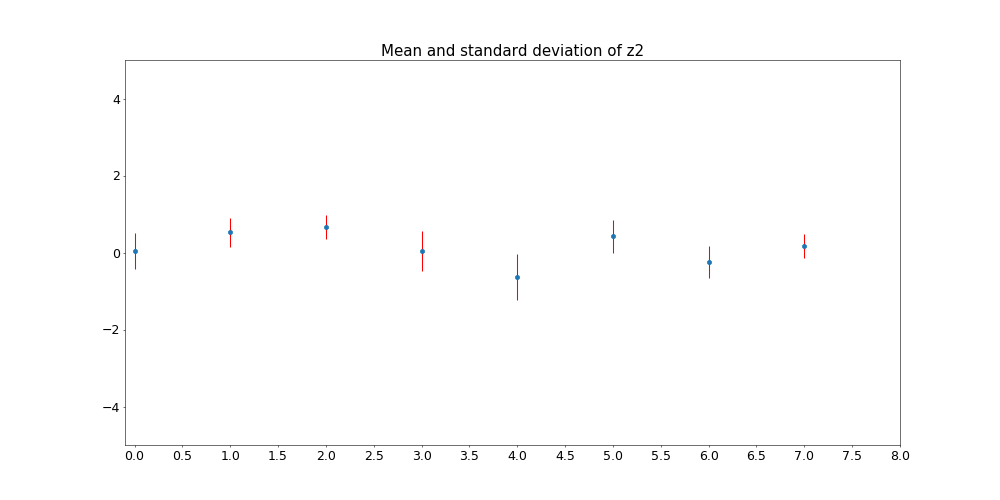
\includegraphics[width=.95\linewidth]{sweep/no_contrast_no_norm_z2_stats.png} 
    \caption{No contrast \newline no norm $\bm{z}_{2}$ statistics} 
    \label{fig:no-contrast-no-norm-stats}
  \end{minipage} 
  \begin{minipage}{0.5\linewidth}
    \centering
    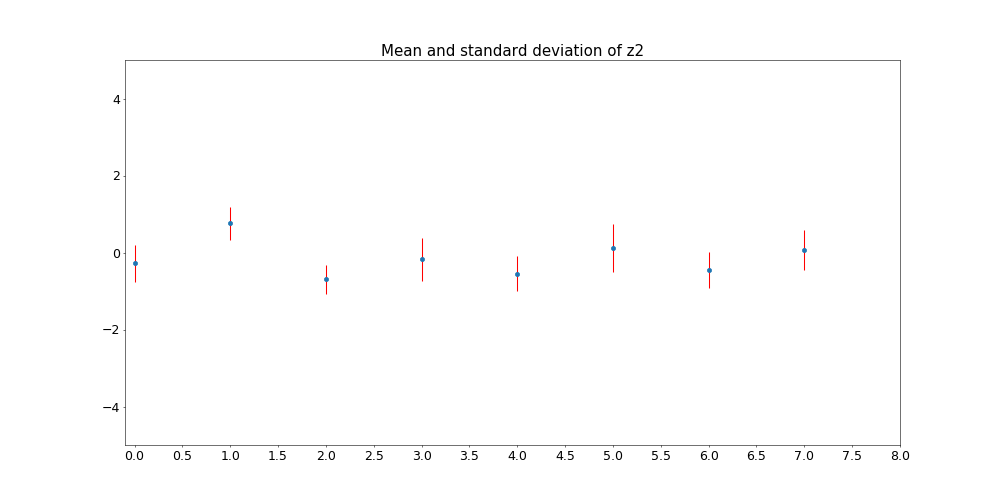
\includegraphics[width=.95\linewidth]{sweep/contrast_no_norm_z2_stats.png} 
    \caption{Contrast, no norm. \newline $\bm{z}_{2}$ statistics} 
    \label{fig:contrast-no-norm-stats}
  \end{minipage}
\end{figure}

\vspace{4mm}

\par With the non-normalized settings in (\ref{fig:no-contrast-no-norm-sweep}) the latent component $4$ is selected from (\ref{fig:no-contrast-no-norm}) with regard to its mean and deviation from (\ref{fig:no-contrast-no-norm-stats}), sweeping therefore in the almost $2\sigma$ range $[-2, 1]$ in the fourth component results in generated samples differing not mostly in contrast but at the bottom \footnote{since generation was done in row flattened order, this means that closer to the right end of the spectrum} of (\ref{fig:no-contrast-no-norm-sweep}) results in a class resembling the $1$st label what we expected (\ref{fig:label-contrast-corr-1}, \ref{fig:label-contrast-corr-2}). However, when contrast is introduced (\ref{fig:contrast-no-norm-sweep-3}, \ref{fig:contrast-no-norm-sweep-5}) still there are high correlations with the one-hot encoded labels, so we could not get a truly disentangled contrast representation in the latent components. On the other hand what we can see in these generated samples that the $3$rd and $5$th components that have high correlation with the random contrast (\ref{fig:contrast-no-norm}) resulted in high contrast images, especially in (\ref{fig:contrast-no-norm-sweep-5}).

\vspace{4mm}

\par Moving on to the normalized scenario:

\vspace{4mm}

\begin{figure}[H] 
  \label{fig:contrast-correlation} 
  \begin{minipage}{0.4\linewidth}
    \centering
    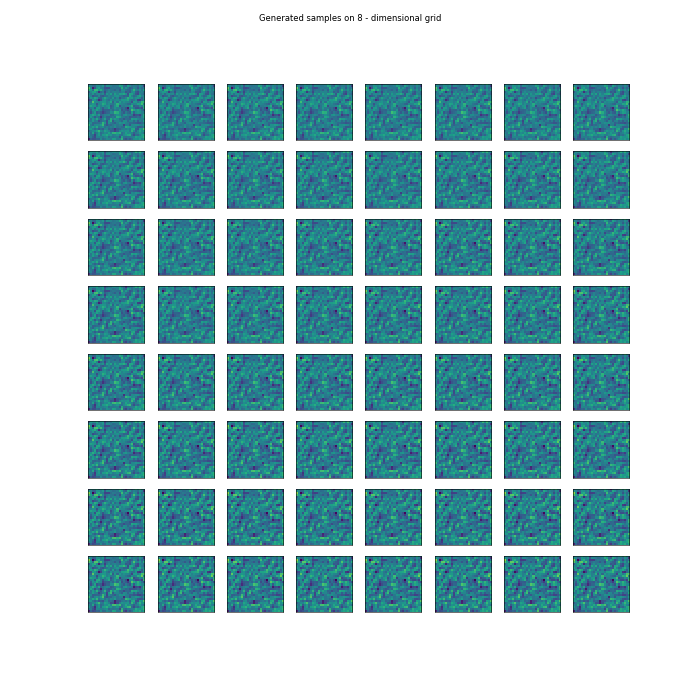
\includegraphics[width=.8\linewidth]{sweep/norm_no_contrast_sweep_one_to_two_4th_param.png} 
    \caption{No contrast, norm., sweep in $[1, 2]$, $4$th compoment} 
    \label{fig:no-contrast-norm-sweep}
  \end{minipage}%%
  \begin{minipage}{0.6\linewidth}
    \centering
    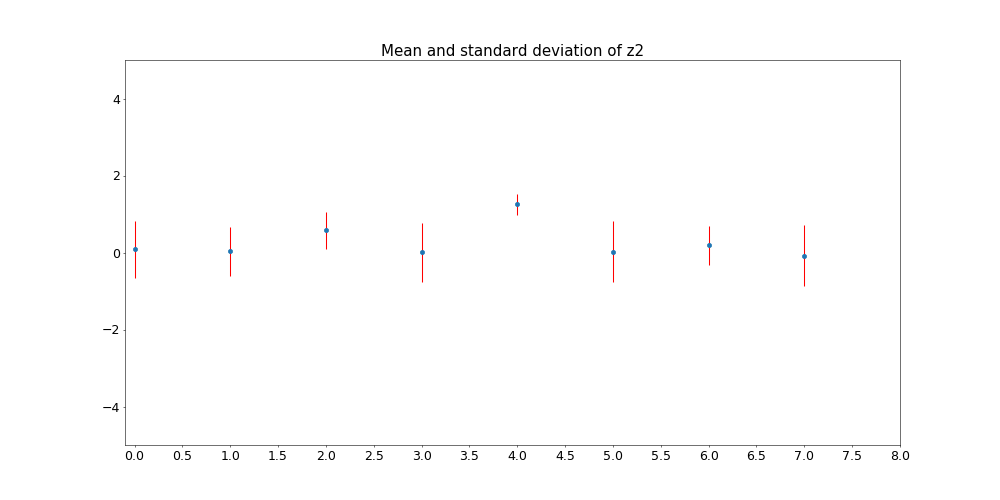
\includegraphics[width=1\linewidth]{sweep/norm_no_contrast_z2_stats.png} 
    \caption{No contrast, norm.,  $\bm{z}_{2}$ statistics} 
    \label{fig:no-contrast-no-norm-stats}
  \end{minipage} 
\end{figure}

\vspace{4mm} 
 
\par  These generated samples with sweeping suggests that the correlations of the $4$th component with the random contrast values in (\ref{fig:no-contrast-norm}) is not high enough, therefore it is not encoding contrast at all. In (\ref{fig:no-contrast-norm-sweep}) there are no trivial differences across the sweep so it is unknown what the component actually encodes. Adding additional contrast to normalized images results in:

\vspace{4mm}
 
\begin{figure}[H]
  \begin{minipage}{0.5\linewidth}
    \centering
    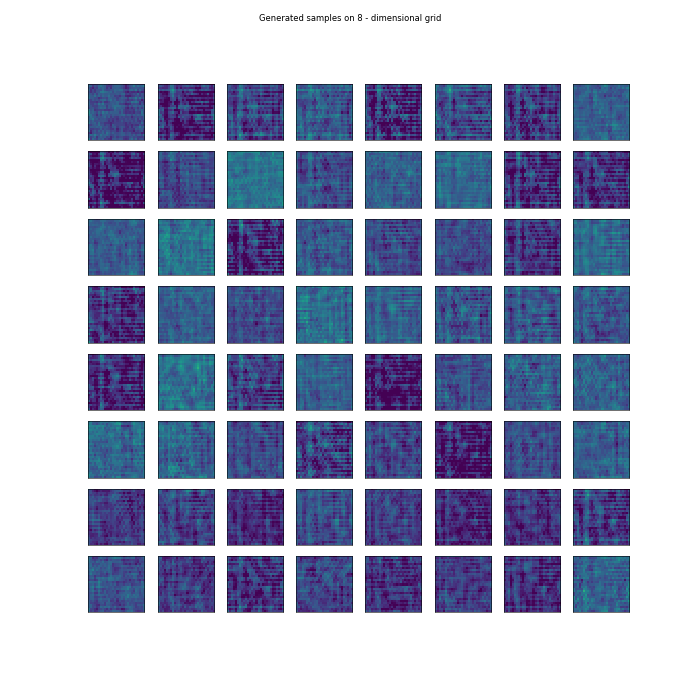
\includegraphics[width=.85\linewidth]{sweep/norm_contrast_sweep_zero_to_one_0th_param.png} 
    \caption{Contrast, norm., sweep in $[0, 1]$ \newline $0$th component} 
    \label{fig:contrast-norm-sweep-0}
  \end{minipage} 
  \begin{minipage}{0.5\linewidth}
    \centering
    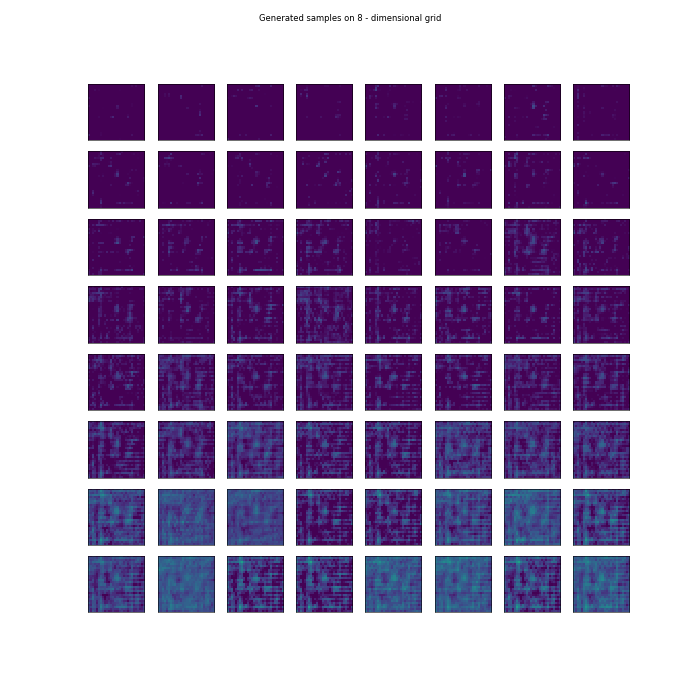
\includegraphics[width=.85\linewidth]{sweep/norm_contrast_sweep_minus_two_to_one_2nd_param.png} 
    \caption{Contrast, norm., sweep in $[-2, 1]$ \newline $2$nd component} 
    \label{fig:contrast-norm-sweep-2}
  \end{minipage}
\end{figure}


\begin{figure}[H]
  \begin{minipage}{0.5\linewidth}
    \centering
    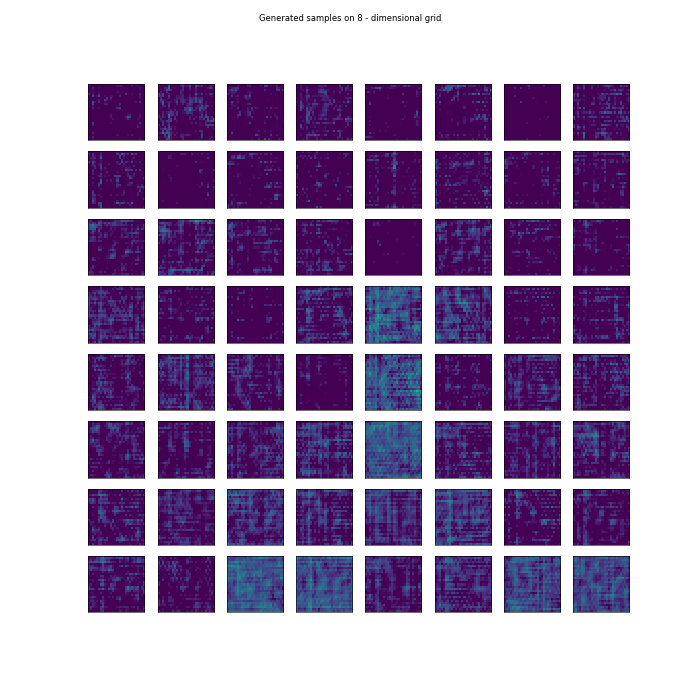
\includegraphics[width=.85\linewidth]{sweep/norm_contrast_sweep_minus_two_to_one_3rd_param.png} 
    \caption{Contrast, norm., sweep in $[-2, 1]$ \newline  $3$rd component} 
    \label{fig:contrast-norm-sweep-3}
  \end{minipage}
  \begin{minipage}{0.5\linewidth}
    \centering
    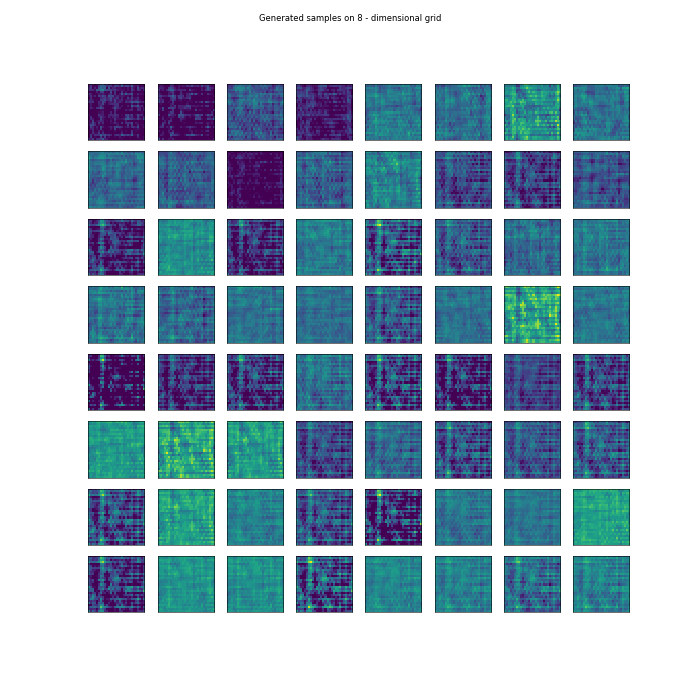
\includegraphics[width=.85\linewidth]{sweep/norm_contrast_sweep_zero_to_two_6th_param.png} 
    \caption{Contrast, norm., sweep in $[0, 2]$ \newline $6$th component} 
    \label{fig:contrast-norm-sweep-6}
  \end{minipage}
\end{figure}

\begin{figure}[H]
    \centering
    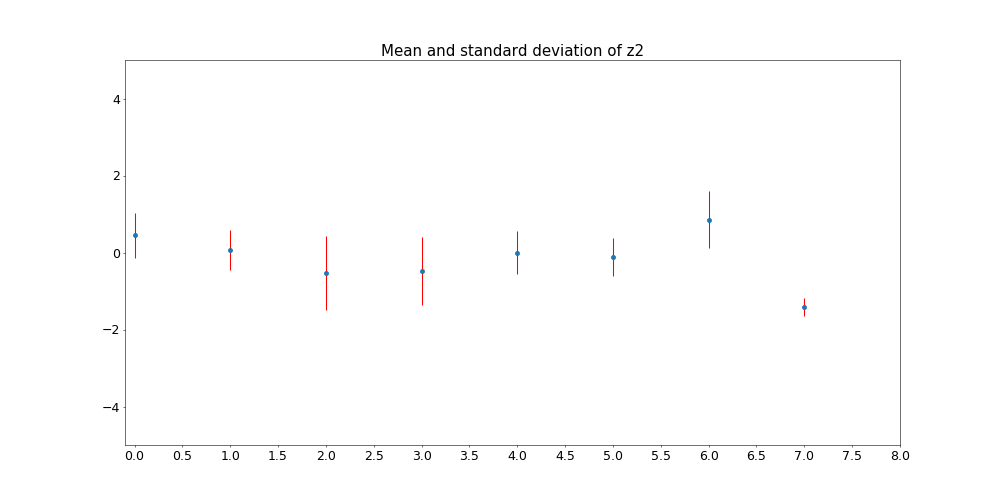
\includegraphics[width=.85\linewidth]{sweep/norm_contrast_z2_stats.png} 
    \caption{Contrast, norm., $\bm{z}_2$ statistics} 
    \label{fig:contrast-norm-stats}
\end{figure}

\vspace{4mm}

\par The components were selected from the corresponding contrast correlation plot (\ref{fig:contrast-norm}) and their ranges very selected from (\ref{fig:contrast-norm-stats}) to approximately cover $2\sigma$ range of the mean. We expect gradual contrast increment in row wise order but this can only be seen vaguely on (\ref{fig:contrast-norm-sweep-2}) but not in the others.

\newpage

\subsection{What is needed to disentangle contrast? Comparison of models}

\vspace{5mm}

\par First of all, it is crucial to properly analyze whether a deep, hierarchical architecture is actually hierarchical. In doing so we must observe the top (in our case the second) layer in our model to check whether the deepest stochastic layer has any effect on the reconstructions by validating means and standard deviations of the sampled distributions that were introduced in (\ref{eq:z1-mean-sigma-1}, \ref{eq:z1-mean-sigma-2}). This is crucial information as we are sampling our model from the deepest stochastic layer and without meaningful top down components (\ref{eq:ladder-vae-sampling}) becomes random noise added to the reconstructions that are encoded by the decoder model and not by stochastic parameters.

\vspace{4mm}

\par Remaining at first layer linear encoders and last layer linear decoders with the ladder VAE architecture and the same added or not added extra contrast, with or without normalization I present some vector visualizations of top down and bottom up mean and variation vectors compared to the $\mu_{z^{(1)}}$ and $\sigma_{z^{(1)}}$.

\vspace{4mm}

\begin{figure}[H]
  \begin{minipage}{0.5\linewidth}
    \centering
    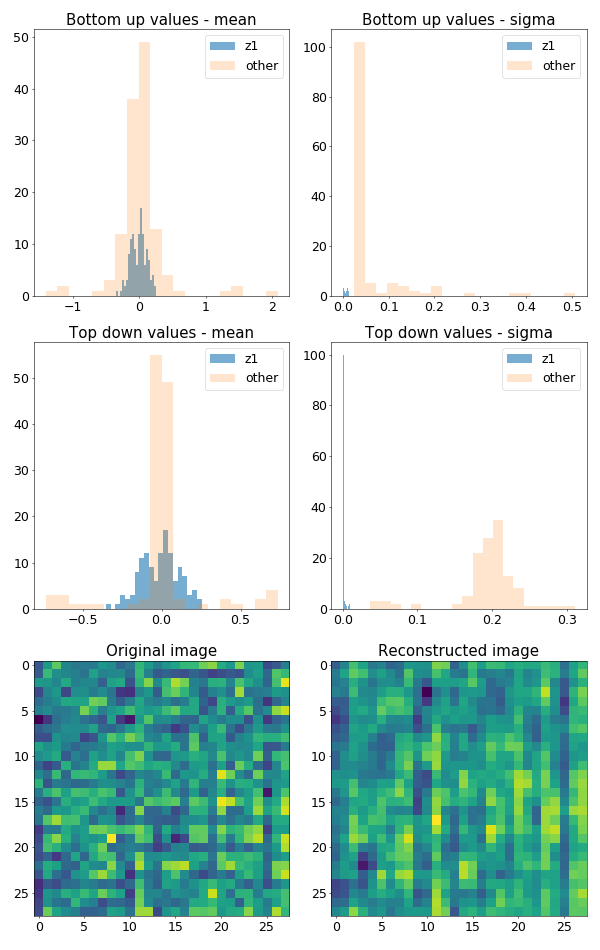
\includegraphics[width=.6\linewidth]{z1_vis/14_DenseLinLinLadderVAE_noContrastNorm_-stats-1_TD_BU_COMPS_1.png}
  \end{minipage}
  \begin{minipage}{0.5\linewidth}
    \centering
    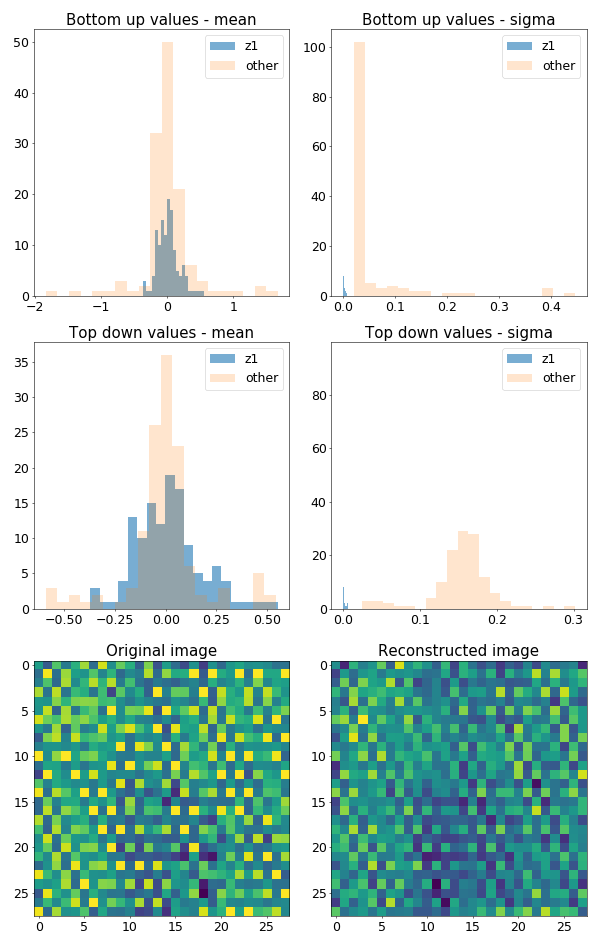
\includegraphics[width=.6\linewidth]{z1_vis/14_DenseLinLinLadderVAE_noContrastNorm_-stats-2_TD_BU_COMPS_1.png} 
  \end{minipage}

  \begin{minipage}{0.5\linewidth}
    \centering
    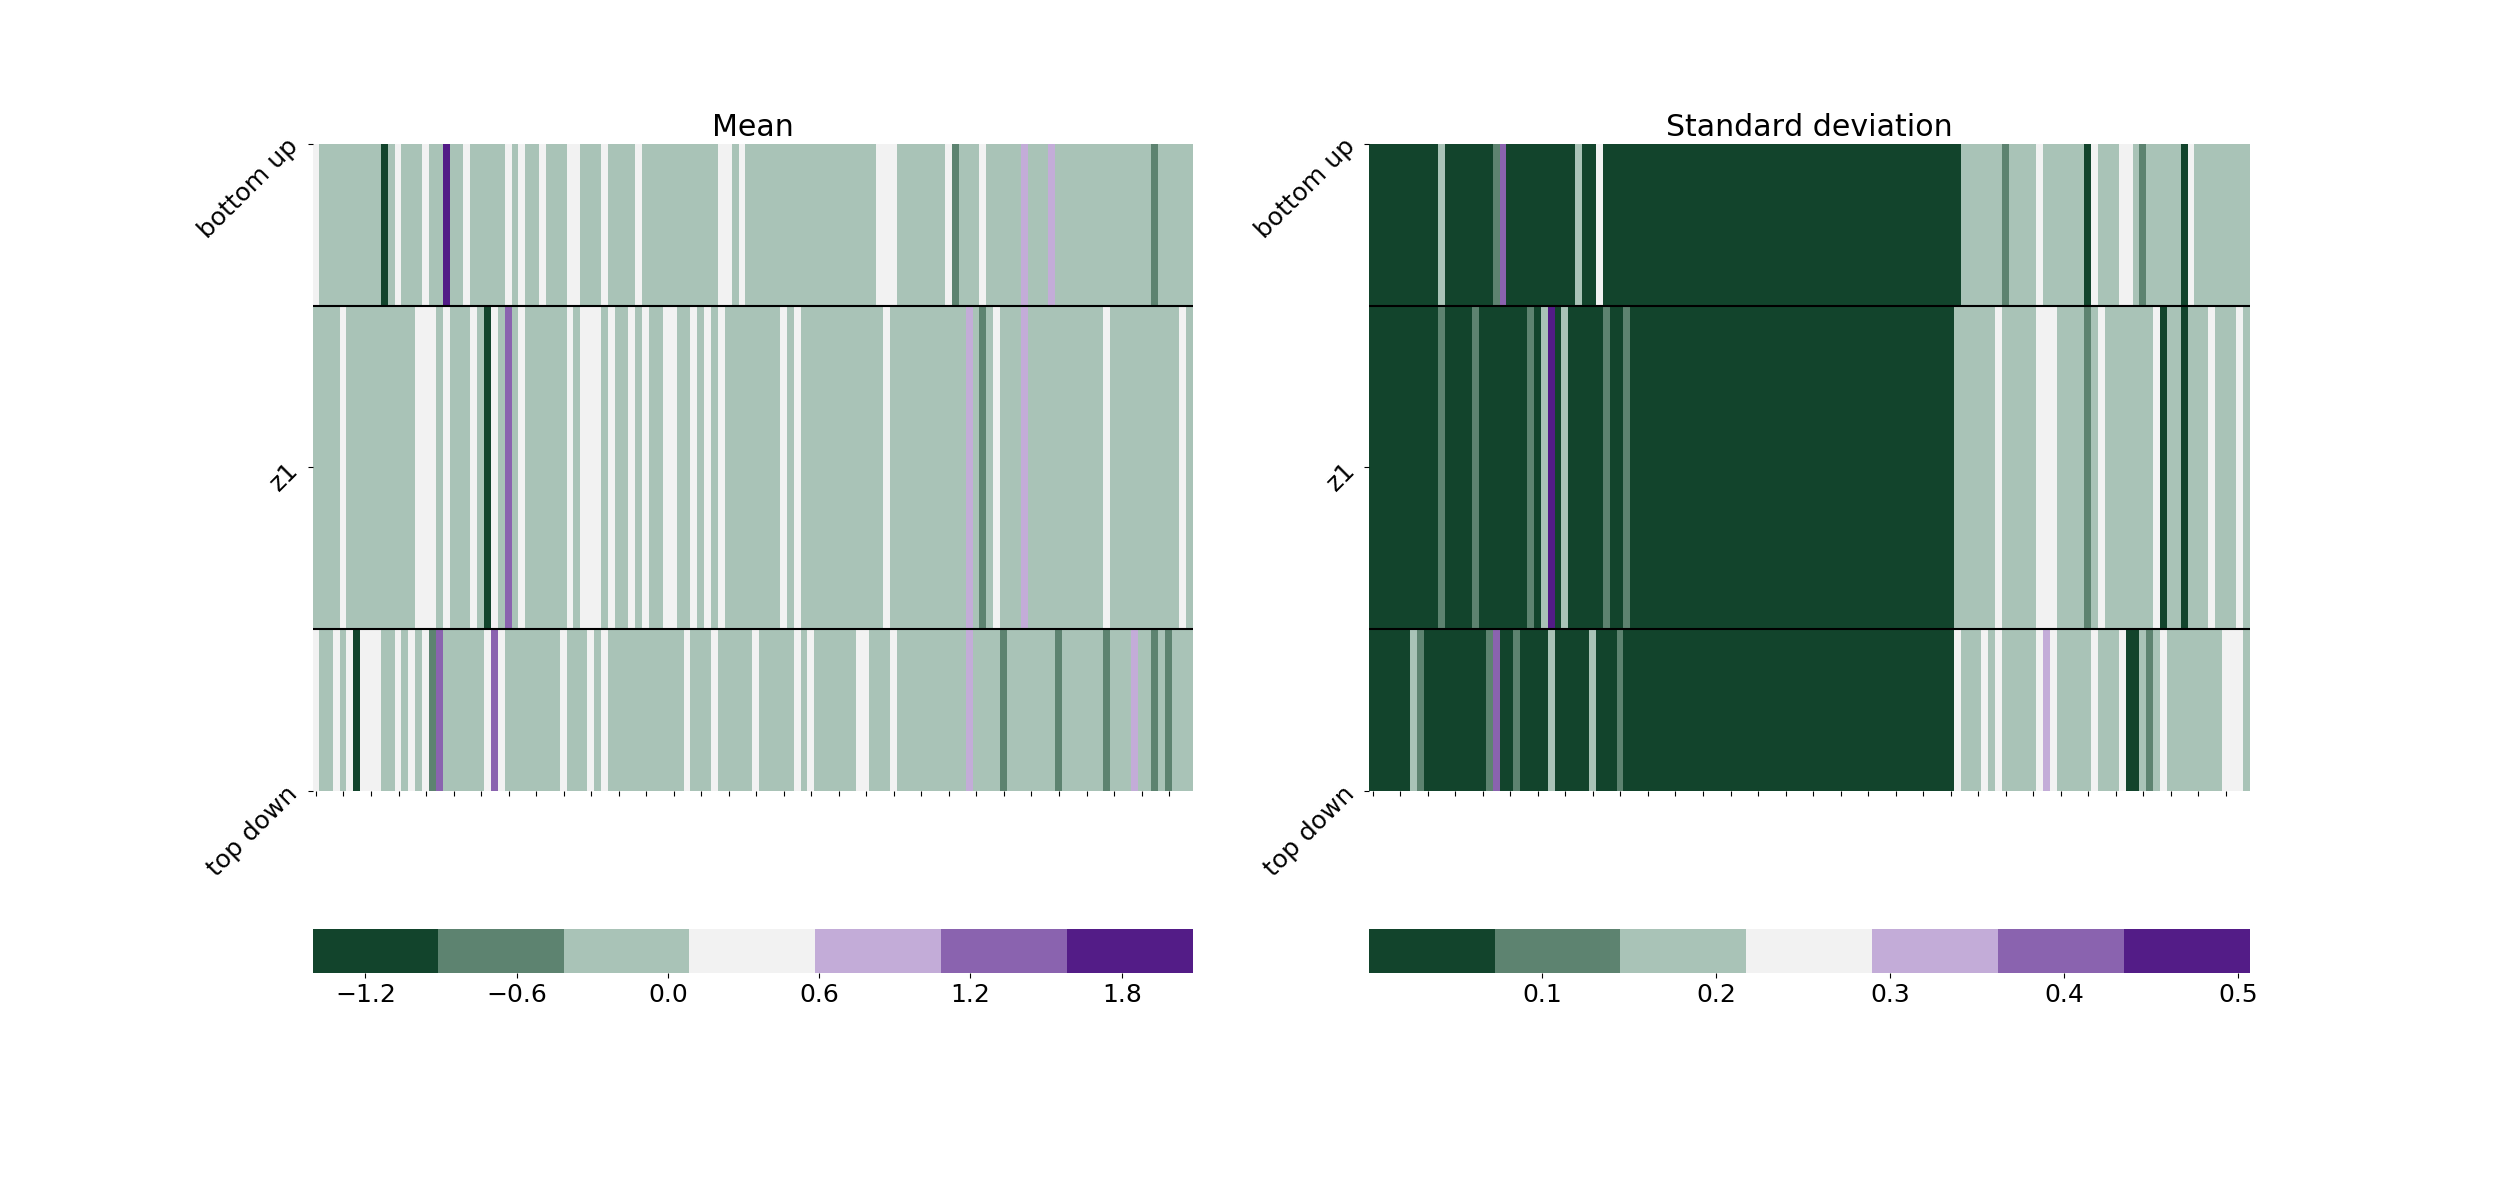
\includegraphics[width=.75\linewidth]{z1_vis/14_DenseLinLinLadderVAE_noContrastNorm_-stats-1_vector_comparisons_1.png} 
    \caption{No contrast, no normalization}
    \label{fig:sample-no-norm-no-contrast-1}
  \end{minipage}
  \begin{minipage}{0.5\linewidth}
    \centering
    \includegraphics[width=.75\linewidth]{z1_vis/14_DenseLinLinLadderVAE_noContrastNorm_-stats-2_vector_comparisons_1.png}
    \caption{No contrast, no normalization}
    \label{fig:sample-no-norm-no-contrast-2}
  \end{minipage}
\end{figure}

\par In (\ref{fig:sample-no-norm-no-contrast-1}) the first two rows of plots show the histograms of the top down, bottom up and actual means and standard deviations where we can observe that the model learns very small standard deviations around 0 (small blue bars). The plot of textures shows the input and the reconstruction of that input right next to it while the last row of plots visualizes the actual vectors with divergent color map to make the differences more pronounced. What we can observe from these is that the means and standard deviations are sparse therefore most of the variables are not encoding information at all meaning that they could be eliminated or smaller latent dimensions could be applied.

\vspace{4mm}

\par In one hand, we can also observe that the top down components are used as well as the bottom up components and the means of the top down components closely approximates the actual mean of $\bm{z}^{(1)}$. One the other hand, the deviation has components with very high values. This is the case in both examples (\ref{fig:sample-no-norm-no-contrast-1}, \ref{fig:sample-no-norm-no-contrast-2}).

\vspace{4mm}

\begin{figure}[H]
  \begin{minipage}{0.5\linewidth}
    \centering
    \includegraphics[width=.6\linewidth]{z1_vis/z1_vis_no_contrast_norm/17_DenseLinLinLadderVAE_contrastNorm-stats-1_TD_BU_COMPS_1.png}
  \end{minipage}
  \begin{minipage}{0.5\linewidth}
    \centering
    \includegraphics[width=.6\linewidth]{z1_vis/z1_vis_no_contrast_norm/17_DenseLinLinLadderVAE_contrastNorm-stats-2_TD_BU_COMPS_1.png} 
  \end{minipage}

  \begin{minipage}{0.5\linewidth}
    \centering
    \includegraphics[width=.75\linewidth]{z1_vis/z1_vis_no_contrast_norm/17_DenseLinLinLadderVAE_contrastNorm-stats-1_vector_comparisons_1.png} 
    \caption{No contrast, normalization}
    \label{fig:sample-norm-no-contrast-1}
  \end{minipage}
  \begin{minipage}{0.5\linewidth}
    \centering
    \includegraphics[width=.75\linewidth]{z1_vis/z1_vis_no_contrast_norm/17_DenseLinLinLadderVAE_contrastNorm-stats-2_vector_comparisons_1.png}
    \caption{No contrast, normalization}
    \label{fig:sample-norm-no-contrast-2}
  \end{minipage}
\end{figure}

\vspace{4mm}

\par From these plots there is no evident effect of normalization on these results. Moving on to added contrast:

\vspace{4mm}

\begin{figure}[H]
  \begin{minipage}{0.5\linewidth}
    \centering
    \includegraphics[width=.6\linewidth]{z1_vis/z1_vis_contrast_no_norm/15_DenseLinLinLadderVAE_textures_noContrastNorm_contrast-stats-1_TD_BU_COMPS_1.png}
  \end{minipage}
  \begin{minipage}{0.5\linewidth}
    \centering
    \includegraphics[width=.6\linewidth]{z1_vis/z1_vis_contrast_no_norm/15_DenseLinLinLadderVAE_textures_noContrastNorm_contrast-stats-2_TD_BU_COMPS_1.png} 
  \end{minipage}

  \begin{minipage}{0.5\linewidth}
    \centering
    \includegraphics[width=.75\linewidth]{z1_vis/z1_vis_contrast_no_norm/15_DenseLinLinLadderVAE_textures_noContrastNorm_contrast-stats-1_vector_comparisons_1.png} 
    \caption{Contrast, no normalization}
    \label{fig:sample-no-norm-contrast-1}
  \end{minipage}
  \begin{minipage}{0.5\linewidth}
    \centering
    \includegraphics[width=.75\linewidth]{z1_vis/z1_vis_contrast_no_norm/15_DenseLinLinLadderVAE_textures_noContrastNorm_contrast-stats-2_vector_comparisons_1.png}
    \caption{Contrast, no normalization}
    \label{fig:sample-no-norm-contrast-2}
  \end{minipage}
\end{figure}

\vspace{4mm}

\par We can observe in (\ref{fig:sample-no-norm-no-contrast-1}, \ref{fig:sample-no-norm-no-contrast-2}) that for some classes adding more contrast helps the bottom up and top down components to better approximate the actual values for the mean and standard deviation. This effect is evident from (\ref{fig:sample-no-norm-no-contrast-2}) where the bottom up values are close not just in the means but in the deviation as well and the top down values correctly approximate the mean vector.

\vspace{4mm}

\par Lastly, for the sake of completeness we present the same results for the normalized, contrasted case:

\vspace{4mm}

\begin{figure}[H]
  \begin{minipage}{0.5\linewidth}
    \centering
    \includegraphics[width=.6\linewidth]{z1_vis/z1_vis_norm_contrast/16_DenseLinLinLadderVAE_textures_contrastNorm_contrast-stats-1_TD_BU_COMPS_1.png}
  \end{minipage}
  \begin{minipage}{0.5\linewidth}
    \centering
    \includegraphics[width=.6\linewidth]{z1_vis/z1_vis_norm_contrast/16_DenseLinLinLadderVAE_textures_contrastNorm_contrast-stats-2_TD_BU_COMPS_1.png}
  \end{minipage}

  \begin{minipage}{0.5\linewidth}
    \centering
    \includegraphics[width=.75\linewidth]{z1_vis/z1_vis_norm_contrast/16_DenseLinLinLadderVAE_textures_contrastNorm_contrast-stats-1_vector_comparisons_1.png}
    \caption{Contrast, normalization}
    \label{fig:sample-norm-contrast-1}
  \end{minipage}
  \begin{minipage}{0.5\linewidth}
    \centering
    \includegraphics[width=.75\linewidth]{z1_vis/z1_vis_norm_contrast/16_DenseLinLinLadderVAE_textures_contrastNorm_contrast-stats-1_vector_comparisons_1.png}
    \caption{Contrast, normalization}
    \label{fig:sample-norm-contrast-2}
  \end{minipage}
\end{figure}

\vspace{4mm}

\par It seems that contrast and normalization further improved top down and bottom up approximations resulting n smaller top don deviations which should be extremely useful during sampling since the mean vector is approximated better than before.

\newpage

\section*{References}
\label{sec:references}
\addcontentsline{toc}{section}{\nameref{sec:references}}
\printbibliography[heading=none]

\end{document}